\documentclass[review]{elsarticle}

\usepackage{lineno,hyperref}
\modulolinenumbers[5]



\usepackage{amsmath,amssymb}
\usepackage{multirow}
\usepackage{graphicx}
\usepackage{algorithm}
\usepackage{algorithmic}
\usepackage{color,soul}
\usepackage{booktabs} % For formal tables
\usepackage{tabularx}
\usepackage{subcaption}
\captionsetup{compatibility=false}
\usepackage{mwe}
\usepackage{commath}
\usepackage{verbatim}
\usepackage{mathtools}
\usepackage{cuted}
\usepackage{flushend}



\journal{Journal of \LaTeX\ Templates}

%%%%%%%%%%%%%%%%%%%%%%%
%% Elsevier bibliography styles
%%%%%%%%%%%%%%%%%%%%%%%
%% To change the style, put a % in front of the second line of the current style and
%% remove the % from the second line of the style you would like to use.
%%%%%%%%%%%%%%%%%%%%%%%

%% Numbered
%\bibliographystyle{model1-num-names}

%% Numbered without titles
%\bibliographystyle{model1a-num-names}

%% Harvard
%\bibliographystyle{model2-names.bst}\biboptions{authoryear}

%% Vancouver numbered
%\usepackage{numcompress}\bibliographystyle{model3-num-names}

%% Vancouver name/year
%\usepackage{numcompress}\bibliographystyle{model4-names}\biboptions{authoryear}

%% APA style
%\bibliographystyle{model5-names}\biboptions{authoryear}

%% AMA style
%\usepackage{numcompress}\bibliographystyle{model6-num-names}

%% `Elsevier LaTeX' style
\bibliographystyle{elsarticle-num}
%%%%%%%%%%%%%%%%%%%%%%%

\begin{document}

\begin{frontmatter}

\title{On the Behaviour of Differential Evolution for Problems with Dynamic Linear Constraints\tnoteref{mytitlenote}}
\tnotetext[mytitlenote]{Fully documented templates are available in the elsarticle package on \href{http://www.ctan.org/tex-archive/macros/latex/contrib/elsarticle}{CTAN}.}

%% Group authors per affiliation:
\author{Elsevier\fnref{myfootnote}}
\address{Radarweg 29, Amsterdam}
\fntext[myfootnote]{Since 1880.}

%% or include affiliations in footnotes:
\author[mymainaddress,mysecondaryaddress]{Elsevier Inc}
\ead[url]{www.elsevier.com}

\author[mysecondaryaddress]{Global Customer Service\corref{mycorrespondingauthor}}
\cortext[mycorrespondingauthor]{Corresponding author}
\ead{support@elsevier.com}

\address[mymainaddress]{1600 John F Kennedy Boulevard, Philadelphia}
\address[mysecondaryaddress]{360 Park Avenue South, New York}



\begin{abstract}
Dynamic constrained optimization problems (DCOPs) have been a focal point for researchers' studies in recent years due to its representation in many real-world problems. Current benchmarks proposed for testing these problems in the continuous spaces are either not flexible in terms of dimention of the problem and the environmental changes settings or they mainly focus on non-linear environmental changes on the objective function, while the dynamism in some real-world problems arise in the constraints and can be emulated with linear constraint changes. The purpose of this paper is to introduce a framework which produce benchmarks in which the dynamic environment is created with simple changes on linear constraints so they will allow to analyze algorithms in DCOPs with a better insight. Changes include rotation and translation of hyperplane for one and multiple linear constraints. Our motivation arise upon some real-world problems like hydro-thermal scheduling problem in which the variable demand or available resources vary over-time and create constraint changes.
Our proposed framework creates dynamic benchmarks that are flexible in terms of number of changes, dimension of the problem and can be applied to test any objective function. 
Different constraint handling techniques will then be applied to test the efficacy of the benchmark. For the purpose of algorithms comparison a method for ranking the algorithms performances is proposed. For the experiments a range of artificial functions and one real-world problem in power system domain has been applied.
The results reveal that with these changes set, there was an observable effect on the performance of the constraint handling techniques. 
\end{abstract}

\begin{keyword}
Benchmarking, benchmark generator, constraint handling techniques, dynamic constrained optimization, 
differential evolution, evolutionary computation.

\end{keyword}


\end{frontmatter}

\linenumbers



\section{Introduction}
\label{sec:Intro}
Dynamic constrained optimization problems (DCOPs) in which the objective function or/and the constraints change over time can be observed in a variety of real world problems. Optimal control of hybrid systems or/and hydro-thermal power scheduling~\citep{deb2007dynamic}(contain both discrete and continuous optimization nature)~\citep{de2008plant} and dynamic systems~\citep{dini2006building}. Applications in continuous spaces include source identification~\citep{liu2008adaptive}, parameter estimation~\citep{prata2006simultaneous} and pattern recognition~\citep{pantrigo2008multi}.
One type of source identification can be the problem of finding the source of contamination in water systems. In this problem the search space changes because the information about the problem is not fully known and can only be gradually revealed when time goes by. An example of parameter estimation problem is to minimize the deviation of the actual robot trajectory from a reference (pre-planned trajectory). The mathematical model can be defined off-line, but the parameter tuning (optimization process) is assumed to be done on-line via experiments.
As another example of DCOPs in continuous spaces, the problem of pattern recognition can be considered. This problem is defined to maximize the income by appropriately choosing mixed grazing strategy. In this case the pattern of change is observed from real-world data.

Multiple algorithms have been designed so far to solve the above-mentioned problems in the area of DCOPs~\citep{ECDCOPs, Nguyen20121,Yaneli2016}. The focus of these papers are either on enhancing dynamic handling mechanisms or constraint handling techniques. Dynamic handling techniques include introducing~\citep{Goh_2009} or maintaining diversity~\citep{Bui2005}, memory-based approaches~\citep{Richter2013} and multi population approaches~\cite{branke2000multi}.
Whereas constraint handling techniques applied in DCOPs include penalty~\citep{CEC09}, repair methods~\citep{Das,bu2017continuous,nguyen2012continuous} and feasibility rules~\citep{ameca2014differential}.
In addition, some papers enhanced both constraint handling and dynamic handling mechanisms~\citep{Nguyen20121,Yaneli2016}.

For testing and comparison of algorithms and techniques always there is a need for a comprehensive benchmark suit that can test algorithms considering a range of characteristics.
Although there are a range of benchmarks proposed to test the relevant algorithms for discrete spaces~\citep{woldesenbet2009dynamic}, and/or multi-objective optimization in dynamic environments~\citep{jiang2017evolutionary}, for continuous spaces in single objective optimization so far, probably the most used benchmark is the proposed benchmark in~\citep{Nguyen20121}. In this benchmark, the dynamic changes are applied by adding time-dependent terms to the objective function and the constraints of one of the functions ($G\_24$) of the static benchmark proposed in CEC 2006~\citep{liang2006problem}. However, there are parameters defined to alter the severity of changes in the environment, this benchmark includes only one objective function and is not applicable to test different functions to consider a range of characteristics. Moreover, the proposed problem is a two-dimensional in size and is not flexible to be applied for larger dimension of the problem.
In addition as the feasible regions of the dynamic constraint function in this benchmark are very large, which might not be sufficiently complicated, Bu et all in~\citep{bu2017continuous}, introduces two variants of this benchmark suit that have a parameter to control the size of the feasible region.

A similar benchmark is proposed in~\cite{zhang2014danger} that is more complicated, and involve different types of DCOP characteristics. However, the problem information, including the number of feasible regions, the global optimum, and the dynamics of each feasible region, is lacking. The lack of such information makes it difficult to measure and analyze the performance of an algorithm.

In terms of having a scalable and flexible benchmark, in the literature there are some benchmark generators proposed. Like in~\citep{li2008benchmark} the generalized dynamic benchmark generator is proposed that is designed with the idea of constructing dynamic environments across binary, real, and combinatorial solution spaces. The search space is constructed from a composition of base functions and the dynamism is obtained by tuning some system control parameters. There are six change types of this system: small step, large step, random, chaotic, recurrent, and recurrent change with noise. Thus, this benchmark generator can present different dynamic properties using these change types.

In~\citep{branke1999memory}, a “moving peaks” benchmark (MPB) is proposed that the dynamic environment is created in such a way to have an artificial multi-dimensional landscape consisting of several peaks, where the height, the width and the position of each peak is altered slightly every time a change in the environment occurs. 
In~\citep{morrison1999test}, considering that the continuous space can be modeled as a “field of cones”, then each cone is adjusted individually to represent different dynamics.
In~\citep{yu2010robust} the MPB was modified so that each peak has its own frequency and severity. In the original MPB, all the peaks are changed at the same frequency and severity. 
In~\cite{liu2008new} two simple unimodal functions were proposed, whose dynamics are caused by a time-dependent parameter.

While all the aforementioned benchmark generators focus on creating dynamic objective functions, in this paper we plan to put our focus on creating dynamic constraints. Our motivation come from characteristic of some real-world problems like scheduling power system problem having dynamic linear constraints (due to the variable demand and available resources over-time). For a better insight about the effects of constraint changes we put the objective function as constant. Indeed, this is the case in some real world problems in which only constraints will change like the problem of hydro-thermal power scheduling~\citep{deb2007dynamic} or in discrete spaces a ship scheduling problem~\citep{mertens2006dyncoaa}.

Our generalized proposed framework can generate benchmarks with different scale of the changes, applicable to be used with any objective function and will be adapted to any number of problem dimension. 
Dynamic changes that can happen in a linear constraint are imposed by the translation and rotation of the constraint's hyperplane.
The examples of these two operations on the constraint that happen in a real-world dynamic environment is: the reduction and increment of demand that happens regularly at power system (hyperplane translation) or changes on the share of each plant power production (hyperplane rotation).
We are confident that our proposed benchmark generator is flexible (frequency and severity of changes and dimension of the problem), simple to implement, analyze, or evaluate and computationally efficient and finally allow conjectures to real-world problems.
 
For testing our proposed benchmark we apply differential evolutionary (DE) algorithm which showed competitive results in dynamic and constrained optimization problems so far~\citep{ameca2018comparison} with different constraint handling techniques and observe how they deal with these changes depending on the magnitude and frequency of changes. 

Our experiments are repeated across some well-known functions (sphere, Rosenbrock, Rastrigin and Ackley), and one real-world problem chosen from the power system domain. 
For the analysis on the performance of the tested algorithms, a ranking procedure is introduced that uses the values of the objective function and the constraint violations for each change in the environment to rank the performance of the algorithms. In addition, the common measure modified offline error is also evaluated for the experiments and the results are investigated.
The results reveal that the frequency and amplitude have a direct correlation with the performance of the constraint handling techniques, as they increase so do the recorded measures. Therefore with imposing simple linear changes we could effectively put the algorithms to struggle and test their performance.

The outline of the paper is as follows. Section~\ref{sec:Prim} introduces a short overview of the problem statement. In Section~\ref{sec:change-setup}, our motivation for benchmarking in DCOPs and our proposed dynamic changes' framework is described. Experimental investigations will be presented in Section~\ref{sec:Experiment} and finally in Section~\ref{sec:conclusion} conclusions and future work are summarized.

\section{Problem statement}
\label{sec:Prim}
In this section a general overview of the problem statement is presented.
\subsection{Dynamic constraint optimization problems}
A dynamic constrained optimization problem (DCOP) is an optimization problem where the objective function and/or the constraints can change over time~\citep{Nguyen20121}. Such an optimization problem ideally must be solved at every time instant $t$ or whenever there is a change in any of the objective function and/or the constraints with $t$. In such optimization problems, the time parameter can be mapped with the iteration counter $\tau$ of the optimization algorithm. Such problems often arise in real-world problem solving, particularly in optimal control problems or problems requiring an on-line optimization~\citep{de2008plant}. From the real-world problems hydrothermal scheduling problem~\citep{zhang2018multi} can be an example of DCOPs in continuous spaces and ship scheduling problem~\citep{Mertens_2006} can be an example of DCOPs in combinatorial problems.

Generally, the problem statement in DCOPs can be defined as follows. 

Find $\vec{x}$, at each time $t$, which: 
\begin{equation}
		\min_{\vec{x}\in F_t\subseteq[L, U]} f(\vec{x}, t)
\end{equation}

where $f:S \rightarrow \mathbb{R}$ is a single objective function, $\vec{x} \in \mathbb{R}^D $ is a solution vector and $t \in N^+$ is the current time, 
\begin{equation}
[L, U]=  \left\lbrace \vec{x} = (x_{1},x_{2},...,x_{D}) \mid L_i \leq x_i \leq U_i, i = 1 \ldots D\right\rbrace
\end{equation}
is called the search space ($S$), where $L_i$ and $U_i$ are the lower and upper boundaries of the $i$th variable,

subject to:
\begin{equation}
\begin{array}{l}
F_{t}=\{ \vec{x} \mid \vec{x} \in [L,U], g_i (\vec{x},t) \le 0, i = 1, \ldots, m,\\
h_j (\vec{x},t) = 0,j = 1, \ldots, p\} \\
\end{array}
\end{equation}
is called the feasible region at time $t$, where $g_i(x, t)$ is the linear $i$th inequality constraint at time $t$ and $h_j(x,t)$ is the $j$th equality constraint at time $t$.

$\forall \vec{x} \in F_t$, if there exists a solution $\vec{x}^* \in F_t$ such that 
$f(\vec{x}^*,t)\leq f(\vec{x},t)$,  then $\vec{x}^*$ is called a feasible optimal solution 
and $f(\vec{x}^*,t)$ is called the feasible optimal value at time $t$. 


\section{Benchmarking in DCOPs}
\label{sec:change-setup}
In this section, first our motivation for testing algorithms that are used for real-world optimization problems that lie in the area of DCOPs is presented. Then a framework is proposed to generate benchmarks for testing the behavior of any algorithms in DCOPs.
\subsection{Motivation based on optimization of real-world problems}
Many real-world problems lie in the area of DCOPs, examples include hydro-thermal scheduling problem~\citep{deb2007dynamic}, source identification~\citep{liu2008adaptive}, parameter estimation~\citep{prata2006simultaneous} and pattern recognition~\citep{pantrigo2008multi}.  Many of these real-world problems have single or multiple linear constraints. Therefore, the relevant benchmark can be as simple as creating some changes in the constraints coefficients that represent changes in different times. 
In real-world problems including power scheduling problem~\citep{morales2014managing}, the conditions in the system will change so we encounter a new objective or constraint for the next time step in the system. 
Traditionally power system optimization problems used offline algorithms. In offline methods, the algorithm iterate on all variables in the cyberspace until they converge before their solutions are applied to the physical grid. While offline algorithms have been widely used in traditional power system applications, they may become inadequate in some future applications that involve a large network of distributed energy resources, especially in the presence of fluctuating loads and volatile renewables~\citep{molzahn2017survey}.
Algorithms proposed in DCOPs solve the whole problem like one single search process that need to be solved on-line. The difference is that the optimization decision is based on each single time separately, and the algorithm does not have the information of the whole time-scale for its optimization process. The problem of power system scheduling is used to test our benchmark. The chosen problem is to minimize the cost of power dispatch of a two-bus power system. More detail about the applied problem is presented in Section~\ref{subsec:powersys}.
 
\subsection{Dynamic changes framework}
In this section first the setup for single and multiple constraint paradigm is explained and then frequency setup in DCOPs will be briefly reviewed.
\subsubsection{Constraint setup}
For emulating the dynamic constraints, simple linear constraints are used for search space modification. Although linear constraints are simple, they used as a representation of some of the real world problem constraints and prevents over-complication of the analysis. The general formulation for the linear constraints are as follows. 
 \begin{equation}
g_i(\vec{x})=\sum\limits_{j=1}^{D} a_j x_j-b_i \le 0 \quad  i \in\{ 1, \ldots, m\} 
 \end{equation}
where $g_i(\vec{x})$ is the $i$th inequality constraint, $a_j$ is the $j$th variable coefficient, $x_j$ is the $j$th decision variable, $b_i$ is the upper limit of the $i$th  constraint and $D$ is equal to the problem dimension.
A general case for one constraint is defined first and then is developed for multiple constraints. 

Two operations are defined for changes on constraint, the first one is related to changes on $b$ coefficient (hyperplane translation) and the second one is changes of $a_i$ coefficients (hyperplane rotation). 
These two changes in the simple linear constraint can happen commonly in real-world problems. In a scheduling power plant problem, the changes of demand or capacity of each production plants including stochastic renewable plants can be an example of hyperplane translation. The changes on the share of each plant to produce overall supply, or the probability of renewable resources production can be an example of hyperplane rotation (these are the coefficient of variables). We believe that our following proposal for creating changes in the environment is generally showing the usual changes in some real-world dynamic problems like power system problem. 
 
\textbf{Hyperplane translation:}
If $a_i$ coefficients is chosen in a way to create a unit normal vector of $\vec{a}$, changes of $b$ will directly show the effects of changing the distance from the optimal point. The distance $d$ of the constraint hyperplane from the origin $0^D$ is given by
$	d=b/\left(\sum\limits_{i=1}^{D} a_i^{2}\right)^{1/2}.$

The constraint bound value ($b(t)$) at time $t$ is obtained by adding a random value to its previous time value ($b(t-1)$) as in Equation~\ref{eq:bvalue}.  
\begin{equation}
\label{eq:bvalue}
	b(t)=b(t-1)+k_{r}
\end{equation}

where 
$k_{r}$
%=rand[0,1](h-l)+l$ 
is chosen uniformly at random within the interval $[lk,uk]$. Table~\ref{tab:Settings-bk} shows an example of these settings for creating different magnitudes of change for single and multiple constraints. 
As Table~\ref{tab:Settings-bk} illustrates in single constraint (experiment 1), the changes of $lk$ and $uk$ will impose small, medium and large changes on the hyperplane translation. The second experiment belongs to the case of these settings for multiple constraint. These values are only samples of constraints boundaries for creating dynamic environment. As mentioned before, we can create multiple benchmarks for testing the algorithms with different scales of the changes based on the problem type. 
The two criteria that will affect the proper choice of the values of $lk$ and $uk$ are the dimension of the problem and the variable ranges. 
\begin{table}[htbp]
\centering
\caption{\small Sample settings for hyperplane translation}
\begin{tabular}{l|lccc}
             &         & b0 & lk    & uk    \\\hline
             & Large   & 0  & -2    & 2     \\
Experiment 1 & Medium  & 0  & -1.4  & 1.4   \\
             & Small   & 0  & -0.75 & 2     \\
\\\hline
             & Const 1 & -1 & -1.2  & 1.2   \\
             & Const 2 & -1 & -1.5  & 1.5  \\
Experiment 2 & Const 3 & -1 & -3    & 3     \\
             & Const 4 & -1 & -4    & 4     \\
             & Const 5 & -1 & -5    & 5    
\end{tabular}
\label{tab:Settings-bk}%
\end{table}

\textbf{Hyperplane rotation:}
In this operation, the changes are created by rotating the hyperplane at each separate time. Random numbers are created in $\in [0,1]$ such that we have a unit normal vector of $\vec{a_i}$.
For any time we randomly select some of the coefficients and swap their values. As in this way $\vec{a}$ is still a unit normal vector, therefore the changes at each time is only related to the rotation and not the translation of hyperplane. 
So by making these changes at each time we will have a rotated hyperplane and we can observe how it will effect the algorithms behaviour. 

In another setting both changes of $a_i$ and $b$ values are considered. In this way in any time we have changes on either $b$ or $a_i$ based on a known probability.

With the current settings of the changes on the linear constraint coefficient, we can observe how the algorithms response to the new modified search space. With the comparisons we will observe which one of the compared algorithms will react faster in order to converge to the optimum after a change occurs. 
The coefficients of the linear constraints are generated through a proposed constraint generator and are then fed to the algorithm. Since the constraint coefficients are random, for a fair algorithms comparison, it is needed that all the generated coefficients for each run be the same for all the algorithms and a per algorithm generation would lead to a difference in compared constraints.
At each change of amplitude, the number of feasible and infeasible solutions will change so that we expect to observe how efficiently the algorithms will manage the new set of constraints within the problem.

In many real-world problems including power market problem, multiple constraints rather than single constraint will define the dynamic environment of the problem. In this case changes are imposed on $b_i$ value of $i$th constraint. In order to avoid complexity, at each time we only change one of the constraints boundaries, and this is aligned with the real-problems that one or a few criteria and not all will change at the new environment condition.   
\subsubsection{Frequency setup}
\label{subsec:FrequencySetup}

The frequency of change ($\tau$) is defined as how often the problem changes. A higher frequency seems to be more difficult for an algorithm to solve the related problem as less time is available at each period to reach the new global optimum~\citep{rohlfshagen2009dynamic}.
In the related literature of DCOPs, the number of fitness evaluations is considered as a criteria to represent how frequently a change occurs~\citep{DCOPS}. After a known number of fitness evaluations, a change will occur (frequency of change). In this paper three different large ($\tau=500$), medium ($\tau=1000$) and small ($\tau=2000$) frequencies of change will be considered.

\section{Differential evolutionary algorithm for dynamic constrained optimization}
In this section differential evolutionary as a competitive algorithm in dynamic optimization and three different common constraint handling techniques are applied and tested to check the efficacy of our proposed benchmark.
\subsection{Differential evolutionary algorithm}
Differential evolution (DE) was first introduced in~\citep{storn1997differential} as a stochastic search algorithm that is simple, reliable and fast and showed competitive results in constraint and dynamic optimization~\citep{ameca2018comparison}. Each vector $\vec{x}_{i, G}$ in the current population (called at the moment of the reproduction as target vector) generates one trial vector $\vec{u}_{i, G}$ by using a mutant vector $\vec{v}_{i,G}$. The mutant vector is created applying $\vec{v}_{i,G}= \vec{x}_{r0,G} + F (\vec{x}_{r1,G} - \vec{x}_{r2,G})$,
where $\vec{x}_{r0,G}$, $\vec{x}_{r1,G}$, and $\vec{x}_{r2,G}$ are vectors chosen at random from the current population ($r0 \neq r1 \neq r2 \neq i$); $\vec{x}_{r0,G}$ is known as the base vector and $\vec{x}_{r1,G}$, and $\vec{x}_{r2,G}$ are the difference vectors and $F>0$ is a parameter called scale factor. Then the trial vector is created by the recombination of the target vector and mutant vector using a probability crossover $CR \in [0,1]$. 

In this paper a simple version of DE called DE/rand/1/bin variant is chosen~\citep{Mezura10a}; where ``rand" indicates how the base vector is chosen (at random in our case), ``1" represents  how many vector differences (vector pairs) will contribute in differential mutation, and ``bin" is the type of crossover (binomial in our case). 
Three different constraint handling techniques including penalty~\citep{tessema2009adaptive}, feasibility rules~\citep{deb2000efficient} and $\epsilon$-constrained~\citep{takahama2005constrained} are chosen to be included as for handling constraint with DE algorithm. With different constraint handling techniques we will observe how these algorithms will respond to the new changes in environment.

In order to make an algorithm in static optimization domain suitable for a dynamic optimization, it is needed that the algorithm be equipped with a mechanism to detect the environment changes and a mechanism to re-act to these changes.
In the literature of DCOPs detecting changes by re-evaluating the solutions is the most common change-detection approach. The algorithm regularly re-evaluates some specific solutions (known as detectors) to detect changes in their function values or/and constraints. Detectors can be part of the population or can be considered separately from the search population~\cite{Nguyen20121}.
We used a simple change detection by re-evaluating the first and middle individual in the population. Thus, the objective function and the constraints will be re-evaluated and checked if there is a difference sensed with the previous calculated values. If there is a change detected then individuals of the population are re-evaluated to avoid obsolete information. 
There are other change detection mechanisms like observing the behaviour (drop of value) of best solutions over a number of generations~\citep{janson2006hierarchical}, or the possibility of change detection based on diversity~\citep{richter2009detecting}. 

Among the desirable features that a search strategy should exhibit
to deal with dynamic optimization are i) diversity creation~\citep{Goh_2009}:
the algorithm must be capable of generating diverse solutions; ii) Diversity Maintenance~\citep{Bui2005}: the algorithm should avoid the convergence of every solution into one single optimum; iii) memory-based approaches~\citep{Richter2013}: some past good solutions may become good start points to find a new global optimum;, and iv) a multi population approaches~\cite{branke2000multi}: with several populations searching in parallel and obeying the above features.

Experimenting different dynamic handling mechanisms is a future topic for this work, but for now we only focus on constraint handling mechanisms and avoid applying dynamic handling mechanisms. 

\begin{algorithm}[t]
\small
\begin{algorithmic}[1]
% \BEGIN
	 \STATE Create and evaluate a randomly initial population $\vec{x}_{i,G}\,\forall i, i=1, \ldots, NP$
   \FOR{$G\gets 1$ to $MAX\_GEN$}
      \FOR{$i\gets 1$ to $NP$}
				\STATE Change detection mechanism ($\vec{x}_{i,G}$)				
				\STATE Randomly select $r0 \neq r1 \neq r2 \neq i$
				\STATE $J_{rand} = randint [1,D]$
				\FOR{$j\gets 1$ to $D$}
					\IF{$rand_j \leq CR$ Or $j = J_{rand}$}
						\STATE $u_{i,j,G} = x_{r1,j,G} + F(x_{r2,j,G} - x_{r3,j,G}) $
					\ELSE
						\STATE $u_{i,j,G} = x_{i,j,G}$
					\ENDIF
				\ENDFOR
                \STATE {Select  $u_{i,j,G}$ or $x_{i,j,G}$ based on the constraint handling technique}
			\ENDFOR
		\ENDFOR
%	\END
\end{algorithmic}
\caption{Dynamic differential evolution (DDE)}
\label{alg:DDE}
\vspace{.1cm}
\end{algorithm}

\subsection{Constraint handling techniques} \label{subsec:comparedAlgs}
In this section applied constraint handling techniques including penalty, feasibility rules and $\epsilon$-constrained are briefly reviewed.

The way the algorithm chooses the best solution is different in every constraint handling technique. 
The way that penalty functions treat with the infeasible solution and the amount of their strictness is largely dependent on the penalization factor. The main idea in this technique is that they try to penalize the objective function for the infeasible solutions. In this paper we used an adaptive penalty function method. In this method information gathered from the search process will be used to control the amount of penalties added to infeasible individuals~\citep{tessema2009adaptive}. As in this paper, we want to test five functions with different scale of objective function, we use a method for penalty that uses the normalized values of objective function. With this we do not have to worry about adjusting the penalty factor for avoiding over or under penalization. For more information about the applied penalty method method we refer to the original paper~\citep{tessema2009adaptive}.
Feasibility rules on the other hand are less strict with the infeasible solutions and only give a higher priority for the feasible solutions to be selected. They are based on three simple rules: i) between two feasible solutions, the one with the highest fitness 
value is selected, ii) if one solution is feasible and the other one is infeasible, the 
feasible solution is selected, iii) if both solutions are infeasible, the one with the lower sum of constraint violation is selected.

The $\epsilon$-constrained method proposed by Takahama et al. ~\citep{takahama2005constrained} is similar to the feasibility rules with the only difference that it is more relaxed with choosing between the infeasible solutions. In this method the solutions will be compared based on their objective values for those that have constraint violation below an epsilon level. Therefore some infeasible solutions that may have good information are treated like feasible solutions. The epsilon level can be adaptive in such a way that for the first generations have larger values and gradually decrease.
This gives the algorithm time for the first generations to have the infeasible solutions and for the last generations it gets more strict to avoid infeasible solutions. 


\section{Experimental investigations}
In this section, experimental setup will be introduced first and the results will be analyzed afterwards.
\label{sec:Experiment}
\subsection{Experimental setup for artificial functions}
\label{subsec:exp-setup}
While comparing algorithms is a straight forward task in static optimization, this is challenging in dynamic optimization problems. Measurements proposed for comparing dynamic algorithms so far, like the most common measure: offline error~\citep{DCOPS}, need optimal solutions for each time as part of their calculations. Although, this may not be as complicated for testing the algorithms with benchmarks (as the optimum values are already known), in real world problems most of the time the optimum for each time period is unknown.

Therefore, for comparing algorithms it is essential to have some measures that does not need optimal solutions as part of their calculation. In the following, we propose and investigate some of the ways to compare the effectiveness of each algorithm without the need for optimal solutions. 

\subsubsection{Time-based objective plot and constraint violation}
\label{subsec:timebasedplots}
One qualitative way that helps compliment the comparison of the algorithms is to plot the objective values and sum of constraint violation for different changes in the environment. These measures collected are averaged across thirty runs which results in the values that are plotted.
The top graph shows the objective values for each algorithm. This measure will represent the differences between the objective function values that are obtained with each algorithm for the last generation before a change in time.
The y-axis represents the values of the objective function and the bottom graph shows a bar chart representing the sum of constraint violations for the corresponding time for each algorithm. 
The values for each algorithm are color coded and plotted against each other.
Figure~\ref{fig:objwCV} represents the objective values and sum of constraint violations for Ackley function for hyperplane translation changes.

\subsubsection{Penalized objective function plot}
Figure~\ref{fig:Ackleypenalize} is based only on comparing the objective values of the algorithms, but in this case the objective values of the algorithms that reach infeasible solutions are penalized. The penalization is in such a way that the objective value of the infeasible solution will be changed to an amount larger than the largest amount among all the feasible solutions of the whole time horizon. 
For having a better resolution and having a more reasonable penalized value we divided the time horizon to 8 smaller scales (Figure\ref{fig:Sphere8}). In this case, the penalized value for the objective function of the infeasible solutions will be chosen on the vicinity of that solution in the smaller scale, and we will have a better representation of the algorithms comparison. 
\subsubsection{Modified offline error ($\text{M\_off}\_e$)}
This measurement is equal to the average of the sum of errors in each generation divided by the total number of generations~\citep{nguyen2012continuous}. Lower values for this measure is preferred and the zero value for offline error indicates a perfect performance~\citep{Nguyen20121}. This measure is defined in Equation~\ref{eq:offlineerror}.

\begin{equation}
\text{M\_off}\_e= \frac{1}{G_{max}} \sum_{G = 1}^{G_{max}} e(G)
\label{eq:offlineerror}
\end{equation}
\noindent where $G_{max}$ is the number of generations computed by the algorithm and $e(G)$ denotes the error 
in the current iteration $G$ (see Equation~\ref{eq:error}):

\begin{equation}
	e(G)= |f(\vec{x}^*,t) - f(\vec{x}_{best,G},t)|
	\label{eq:error}
\end{equation}

\noindent where $f(\vec{x}^*,t)$ is the feasible global optima\footnote{This global optima is an approximation, which is the best solution found by DE for large number of evaluations at the current time.} at current time $t$, and $f(\vec{x}_{best,G},t)$ represent the best solution (feasible or infeasible) found so far at generation $G$  (for common offline error) at current time $t$. However for this modified version, in the case where the best solution is infeasible, the worst solution in the population is chosen instead of the best found. The worst solution is selected from an infeasible population as an effort to overtly encourage feasible solutions. The reason for choosing the modified offline error was because in the common offline error, constraint violation is not considered, while here our focus is to observe which one deals with the constraints more effectively.  

\subsubsection{Ranking mechanism}
We propose a measure for ranking the algorithms that does not need optimal solutions and is based on the feasibility rules~\citep{deb2000efficient} using the following procedures. Considering the best solution obtained before a change in time, if two algorithms have feasible solutions, the one with a lower objective function value is the winner. If one of them has infeasible solution and the other one has a feasible one, the algorithm with feasible solution is the winner. If both of them have infeasible solutions, the one with lower sum of constraint violation will win. 
In this way, we can compare the ability of each algorithm to see how they reach the optimal solution in a limited number of evaluations.


 \begin{figure*}[t!]
        \centering
                \begin{subfigure}[b]{0.48\textwidth}   
            \centering            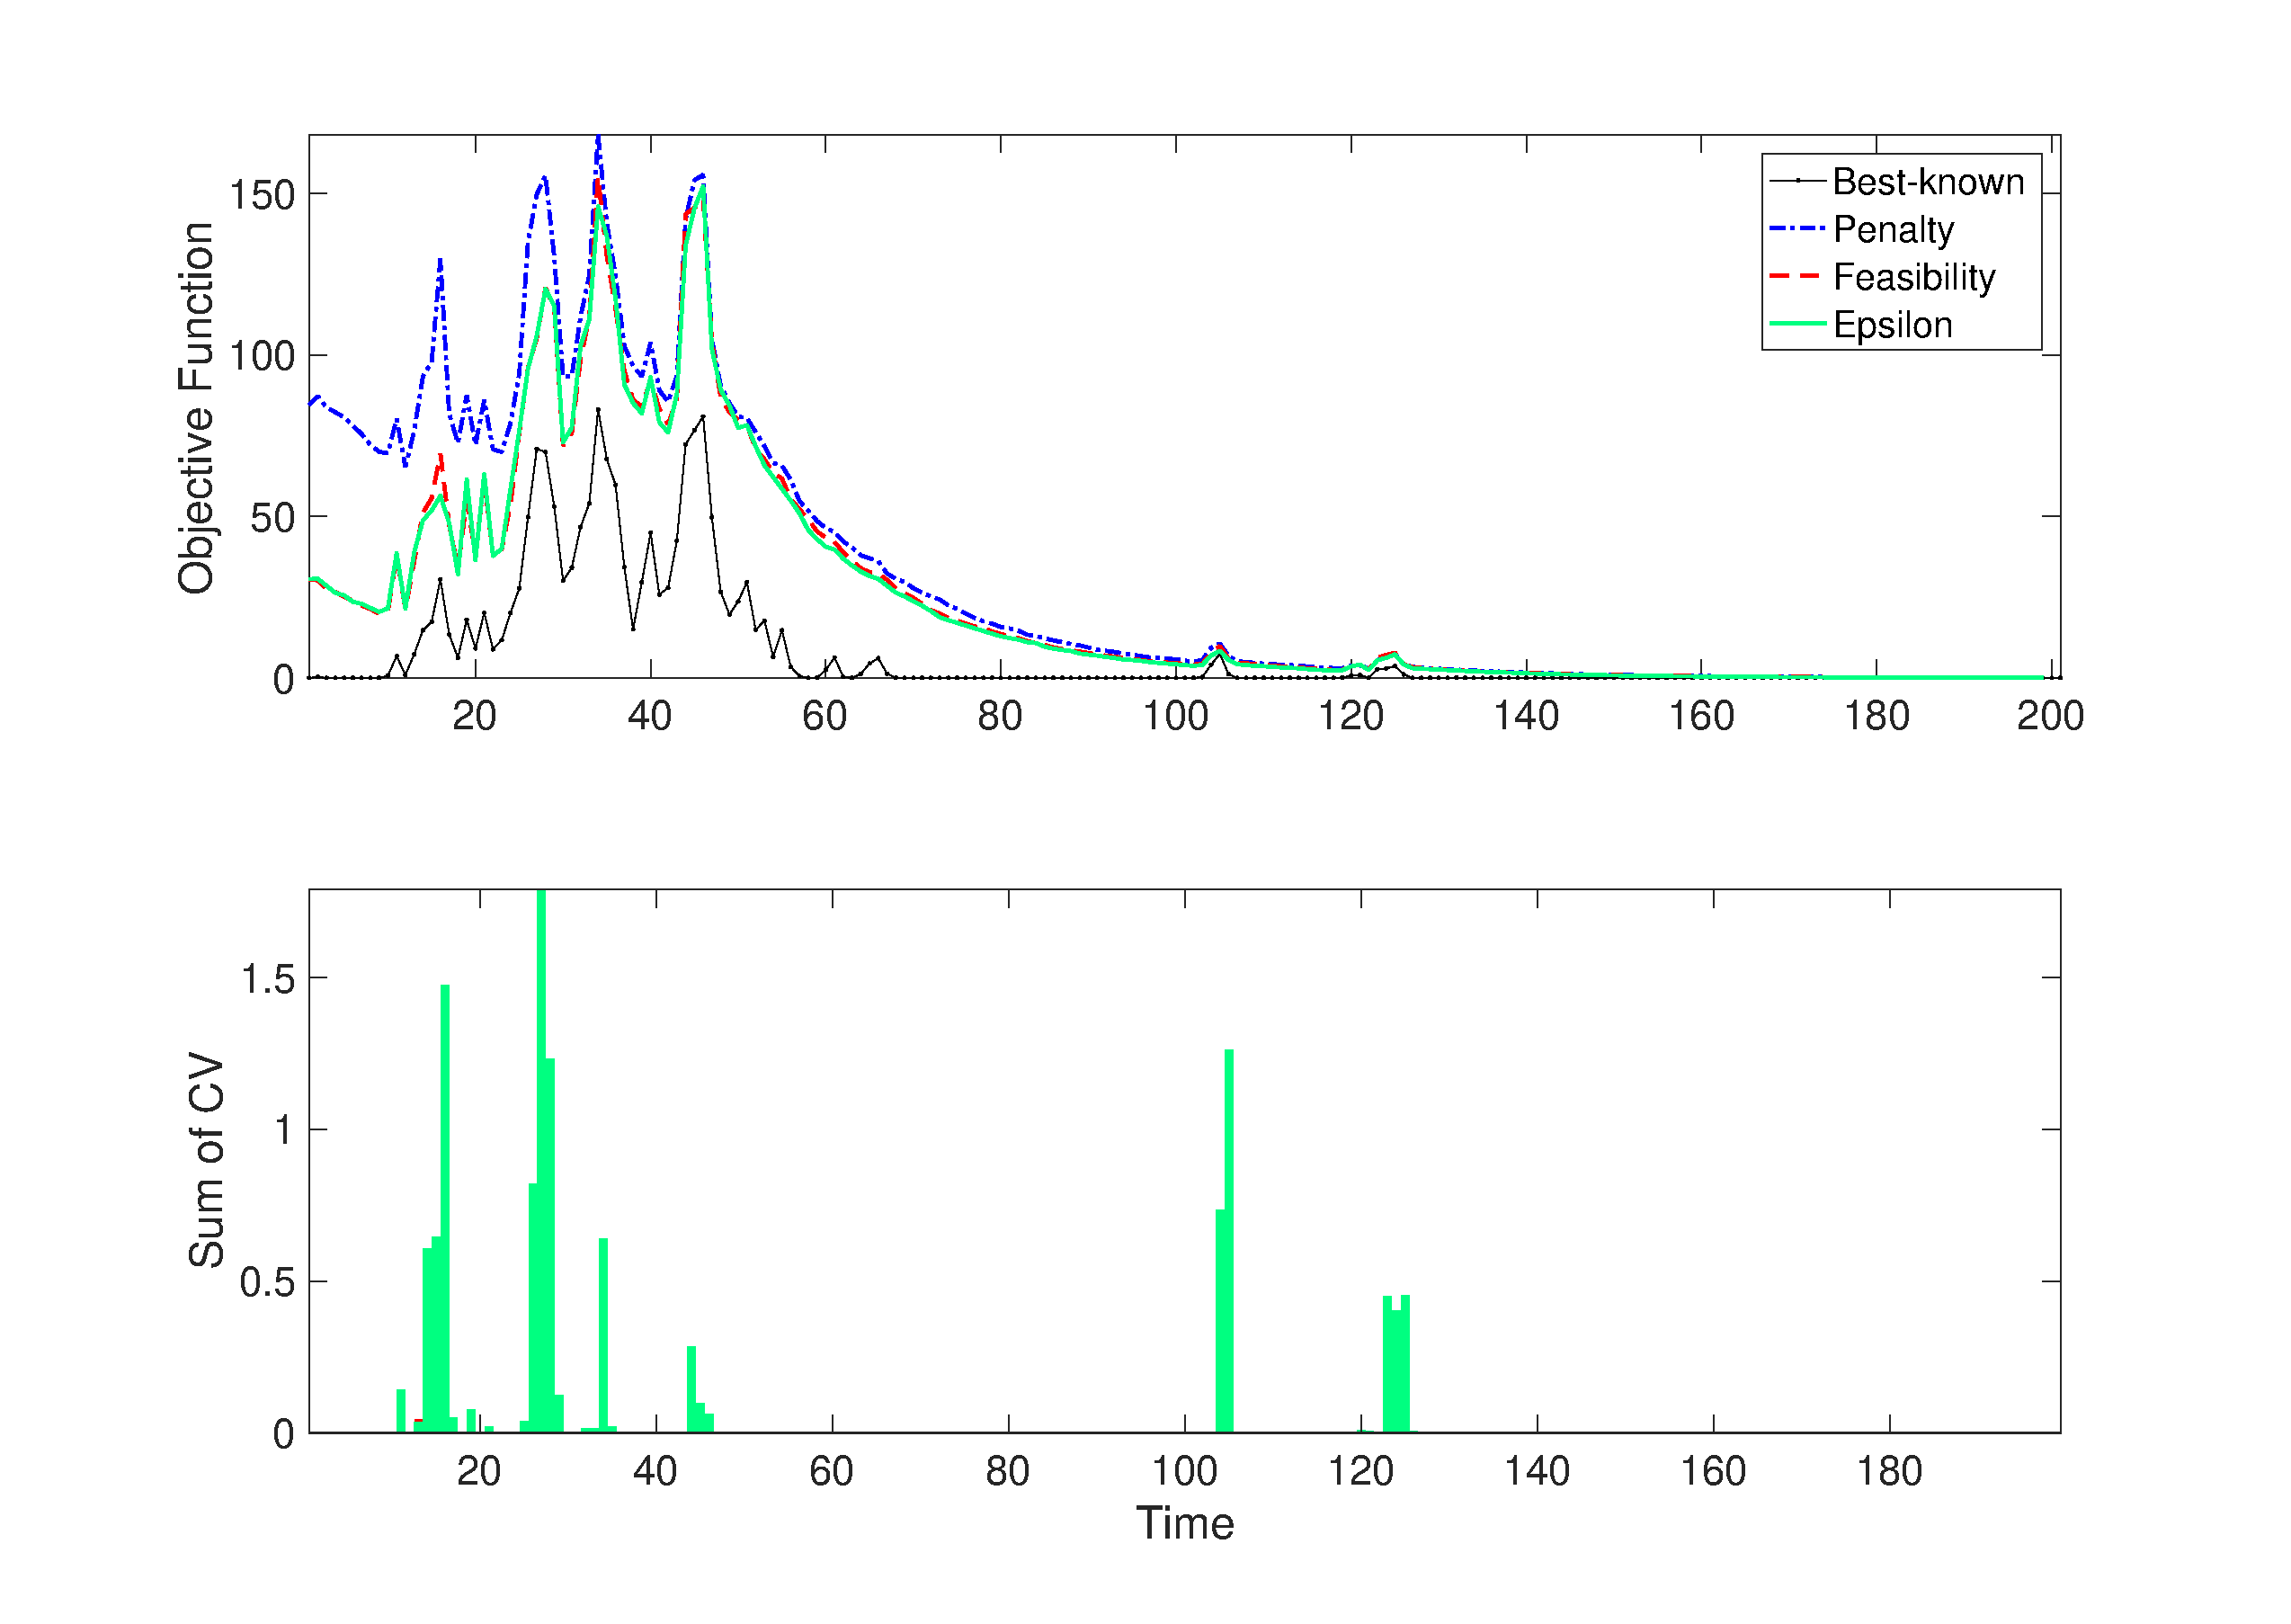
\includegraphics[width=\textwidth,  height=5cm]{figs/freq50Sp.eps}
            \caption[]%
            {{\small Extra large ($\tau$=50)}}    
            \label{fig:freq50}
        \end{subfigure}
        \begin{subfigure}[b]{0.48\textwidth}
            \centering        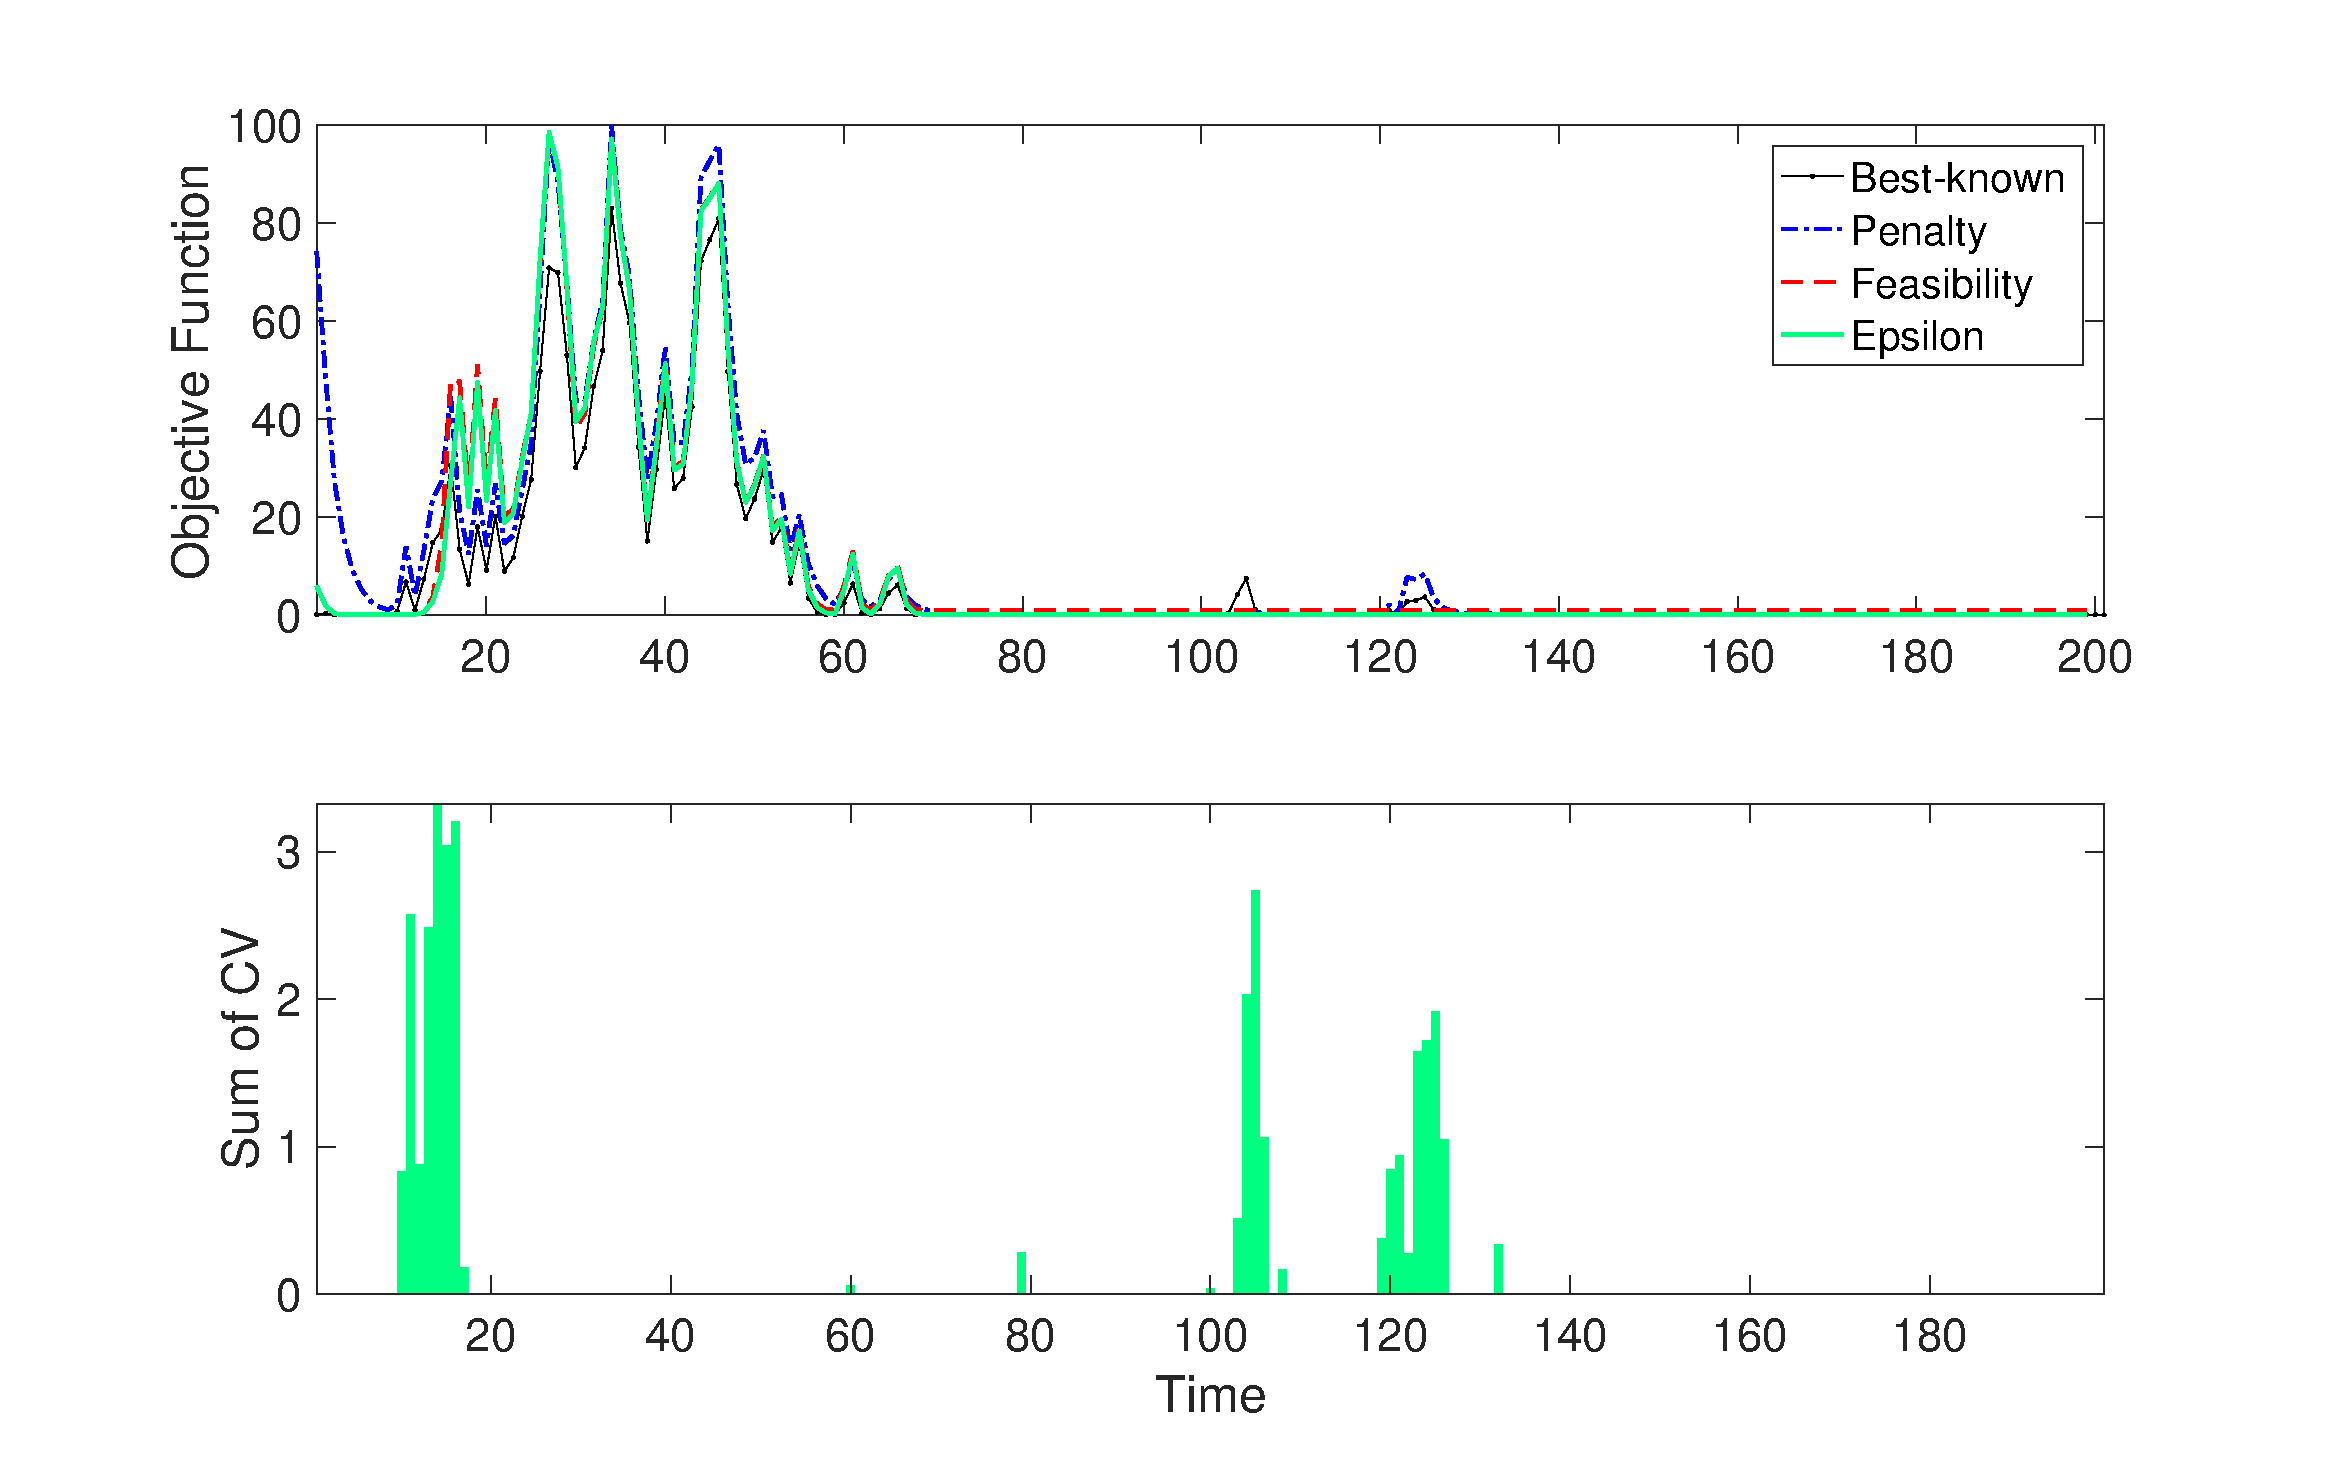
\includegraphics[width=\textwidth,  height=5cm]{figs/freq1000Sp.eps}
            \caption[]%
            {{\small Medium ($\tau$=1000)}}    
            \label{fig:freq1000}
        \end{subfigure}
        %\vskip\baselineskip            
        \caption[]
        {\small Sphere time-based plot for hyperplane translation (average of 30 runs),~\ref{fig:freq50}) extra large $\tau$ ~\ref{fig:freq1000}) medium $\tau$} 
        \label{fig:freqchanges}
    \end{figure*}
\subsubsection{Analytical test setup}
The algorithm ranking procedure explained in Section~\ref{subsec:exp-setup} was applied across every test conducted for analytical testing. In each time change, the performance of the algorithms are ranked and these scores are combined into an overall performance score, fitness values with a constraint violation greater than zero were not considered. Once the overall scores are calculated, the algorithms are ranked in order of the performance. These values are provided alongside the average fitness and constraint violation values paired with their respective standard deviations across runs. We applied this ranking procedure for three algorithms although it is adaptable to be used for comparing any number of algorithms (multi-compare).
The experiments are conducted for different magnitudes of hyperplane translation (experiment 1), a combination of hyperplane rotation and translation (experiment 2), a case using multiple constraints (experiment 3) and dynamic frequency (experiment 4). The results are repeated for four artificial functions. Moreover, power system problem is also tested with our benchmark. For the first three experiments, medium frequency ($\tau=1000$) is applied. For the fourth experiment, large magnitude for hyperplane translation (changes on $b$ value) is chosen.
Parameters of DE are chosen as $NP=20$, $CR=0.2$ and $F$ is a random number in $\in[0.2,0.8]$. The dimension of the problem is 30.

\subsection{Experimental setup for power system problem}
\label{subsec:powersys}
Among real-world problems that lie on the area of DCOPs the scheduling of power system problem is chosen to test our benchmark. In this section after an introduction of the importance of this problem type, the specification of this problem including the objective function, the constraints and the variables will be reviewed. However, the interested reader for more information is referred to Section 5.3.5 of this book~\citep{morales2014managing}.

The integration of an increasing number of renewable resources production in electricity generation systems has resulted in a new circumstance which consists of a large number of stochastic production capacity. Therefore the new production capacity is dependent of stochastic phenomena (e.g., wind level or solar radiation intensity) and not on the will of the owner of such capacity. The exploitation of this renewable capacity whose generation cost is generally low requires the availability of flexible production capacity as a backup, i.e., as reserve. Such flexible capacity ensures the production consumption balance regardless of the output from the stochastic sources. Therefore, the problem of scheduling reserve and production capacities based on the probability scenarios of renewable resources has become an interesting topic in power system domain. As this problem lies on the area of DCOPs, we apply our algorithm and show the effectiveness and the insight behind our proposed benchmark for testing this kind of problem. The mathematical formulation for the objective function and the constraints are briefly reviewed as follows. The schematic of the two bus power system problem is shown at Figure~\ref{fig:powersysp}.
Objective function of this problem given at Equation~\ref{eq:objpowersys} includes (as in order in the equation) dispatch cost, up and down regulation reserve cost, re-dispatch cost, cost of up and down regulation reserve from hydro, cost of load shedding and wind spillage.

\begin{equation}
\label{eq:objpowersys}
 \begin{multlined}
f(\vec{x})=\sum_{k}{c(k)po(k)+C_{up}(k)r_{
up}(k)+C_{dw}(k)r_{dw}(k)}+\\
\sum_{w}{p(w)(
b_{up}(k)y_{up}(k,w)-b_{dw}(k)y_{dw}(k,w))}+\\
\sum_{h}{Ch_{up}(h)rh_{
up}(h)+Ch_{dw}(h)rh_{dw}(h)}+\\
\sum_{i,w}{p(w)(V_{lol} l_{sh}(i,w)+V_{sp} w\_sp(i,w))}
 \end{multlined}
\end{equation}

Variable set includes day-ahead dispatch ($po$), day-ahead hydro power dispatch ($po_h$), day-ahead wind power dispatch ($ws$), reserve for up and down regulation ($r_{up}$, $r_{dw}$), hydro reserve for up and down regulation ($rh_{up}$, $rh_{dw}$), up and down regulation re-dispatch ($y_{up}$, $y_{dw}$), up and down regulation hydro re-dispatch ($yh_{up}$, $yh_{dw}$), load shedding ($l_{sh}$), wind spillage ($w_{sp}$), day-ahead voltage ($\delta_0$), balancing market voltage ($\delta$). The used parameters are as follows: $MN(i,j)$ a binary that shows the connection status of node $i$ and $j$, $b(i,j)$ per unit susceptance of line $i$ and $j$, $p(w)$ scenario probability, $V_{lol}$ value of lost load, $V_{sp}$ value of spilled wind. Some of the indexes used are: $k$ represent power production units, $h$ hydro unit and $w$ scenario.
The constraint set (see Table~\ref{tab:Constraints}) includes multiple linear constraints and is divided to two categories: day-ahead and balancing market constraints. Each of the categories include power balance equality, lower and upper bounds of capacities, transmission capacity, regulation capacities, load shedding and wind spillage upper bounds. From these constraints, only the power balance for day-ahead and balancing market are equality constraints, the others are inequality constraints.

In this problem, the constraints that have dynamic behaviour belong to demand (both node one and two), wind power production forecast (both scenario one and two) and maximum dispatch of wind power. Therefore, among the set of constraints (see Table~\ref{tab:Constraints}) only the constraints 1, 4, 6, 9 and 10 will have a dynamic nature.


  \begin{figure}[t]
        \centering          
\includegraphics[width=0.6\textwidth, height=5cm]{powersys.png} 
        \caption[]
        {\small Two-bus power system problem}
         \label{fig:powersysp}
    \end{figure}


\begin{table}[t]
\footnotesize
\caption{Constraints Set}
\centering
\begin{tabular}{p{4cm}|p{8cm}}%11.5cm
Constraint name                                  & Mathematic formulation  \\\hline
1-Day-ahead power balance                         &    $\sum_{k}{MG(i,k)x(k)}+\sum_{h}{MH(i,h)x(h)}+ws(i)-\sum_{j|(MN(i,j)=1)}{b(i,j)(\delta_0(i)-\delta_0(j))}=d(i)$                     \\\hline
2-Day-ahead capacity upper and lower bound        &    $x+r_{up} \le Pmax$ , $x-r_{dw} \geq Pmin$                    \\\hline
3-Upper and lower bound for hydro schedule        &    $xh+rh_{up} \le Phmax$ , $xh-rh_{dw} \geq Phmin$                      \\\hline
4-Upper bound for wind schedule                   &    $ws \le Wsmax$                     \\\hline
5-Day-ahead transmission capacity                 & If ($MN(i,j)=1$):   $b(i,j)(\delta_0(i,w)-\delta_0(j,w)) \le Tmax(i,j)$                   \\\hline
6-Balancing market power balance                  &              $\sum_{k}{MG(i,k)(y\_up(k,w)-y\_dw(k,w))}+\sum_{h}{MH(i,h)(y\_up(h,w)-y\_dw(h,w))}+l_{sh}(i,w)+
wp(i,w)-ws(i)-w_{sp}(i,w)-\sum_{j|(MN(i,j)=1)}{b(i,j)(\delta(i)-\delta(j))}=-\sum_{j|(MN(i,j)=1)}{b(i,j)(\delta_0(i)-\delta_0(j))}$       \\\hline
7-Regulation capacity upper and lower bound       &     $y_{up} \le r_{up}$ , $y_{dw} \le r_{dw}$                   \\\hline
8-Hydro regulation capacity upper and lower bound &        $yh_{up} \le rh_{up}$ , $yh_{dw} \le rh_{dw}$                   \\\hline
9-Load-shedding upper bound                       &   $l_{sh} \le d$                      \\\hline
10-Wind-spillage upper bound                       &    $w_{sp} \le wp$                     \\\hline
11-Balancing market transmission capacity          &If ($MN(i,j)=1$):   $b(i,j)(\delta(i,w)-\delta(j,w)) \le Tmax(i,j)$                        \\                        
\end{tabular}
\label{tab:Constraints}
\end{table}

\subsection{Experimental results}
In this section, first convergence plot results are explained, then the analytical test results are presented. 

\subsubsection{Remarks on plots}
In all the figures, the dot coded plots show the best-known solution which is counted by running a high enough number of evaluation (one million) with a DE algorithm with feasibility rules as constraint handling technique and for each time separately. 

Figure~\ref{fig:freqchanges} illustrates an example of the algorithms behaviour with the changes of the objective function and the constraint violation for extra large and medium frequencies of change. As explained in Section~\ref{subsec:timebasedplots} the objective function and the relevant constraint violation at each time belongs to the last best solution achieved with each algorithm right before a change occurs. As Figure~\ref{fig:freq50} proves for extra large frequency, the algorithms do not have sufficient time to track the optima after a change occurs. While for medium frequency they have more time to converge to the optima more closely. Figure~\ref{fig:objwCV} shows the best solution for each time averaged across all of the runs in the Ackley function with medium frequency ($\tau=1000$) and large amplitude of hyperplane translation changes. As the figure shows, the algorithms managed to track larger changes earlier on in the first times (that happen to belong to the larger magnitude of changes) but the smaller changes were harder to track. This lead to feasibility and $\epsilon$-constrained to become stuck in local optima, unable to track constraint changes. This behavior occurs in multi-modal functions where there are local optima that can trap algorithms which have no obvious way to improve without a good dynamic handling mechanism which these test algorithms lack.
Figure~\ref{fig:Sphere8} shows that these test algorithms can eventually adapt to constraint changed. However, some changes cause them to struggle and it takes considerable time for them to catch up.
The previous mentioned figures are plotted for an average values over all runs. Figure~\ref{fig:Ackleyruns} however, illustrates an example of plotting objective function of Akhley function for each run separately. As this figure proofs variances over all the runs are quiet small and so average is a fair representation of depicting the results.
Figure~\ref{fig:posysresult} shows that although the test algorithms struggled to perform in a real-world problem, the benchmark can be used to analyze algorithm performance with these real-world problems. Our focus for this benchmark is that real-world problems can be applied and analyzed. 
 \begin{figure*}[t!]
        \centering          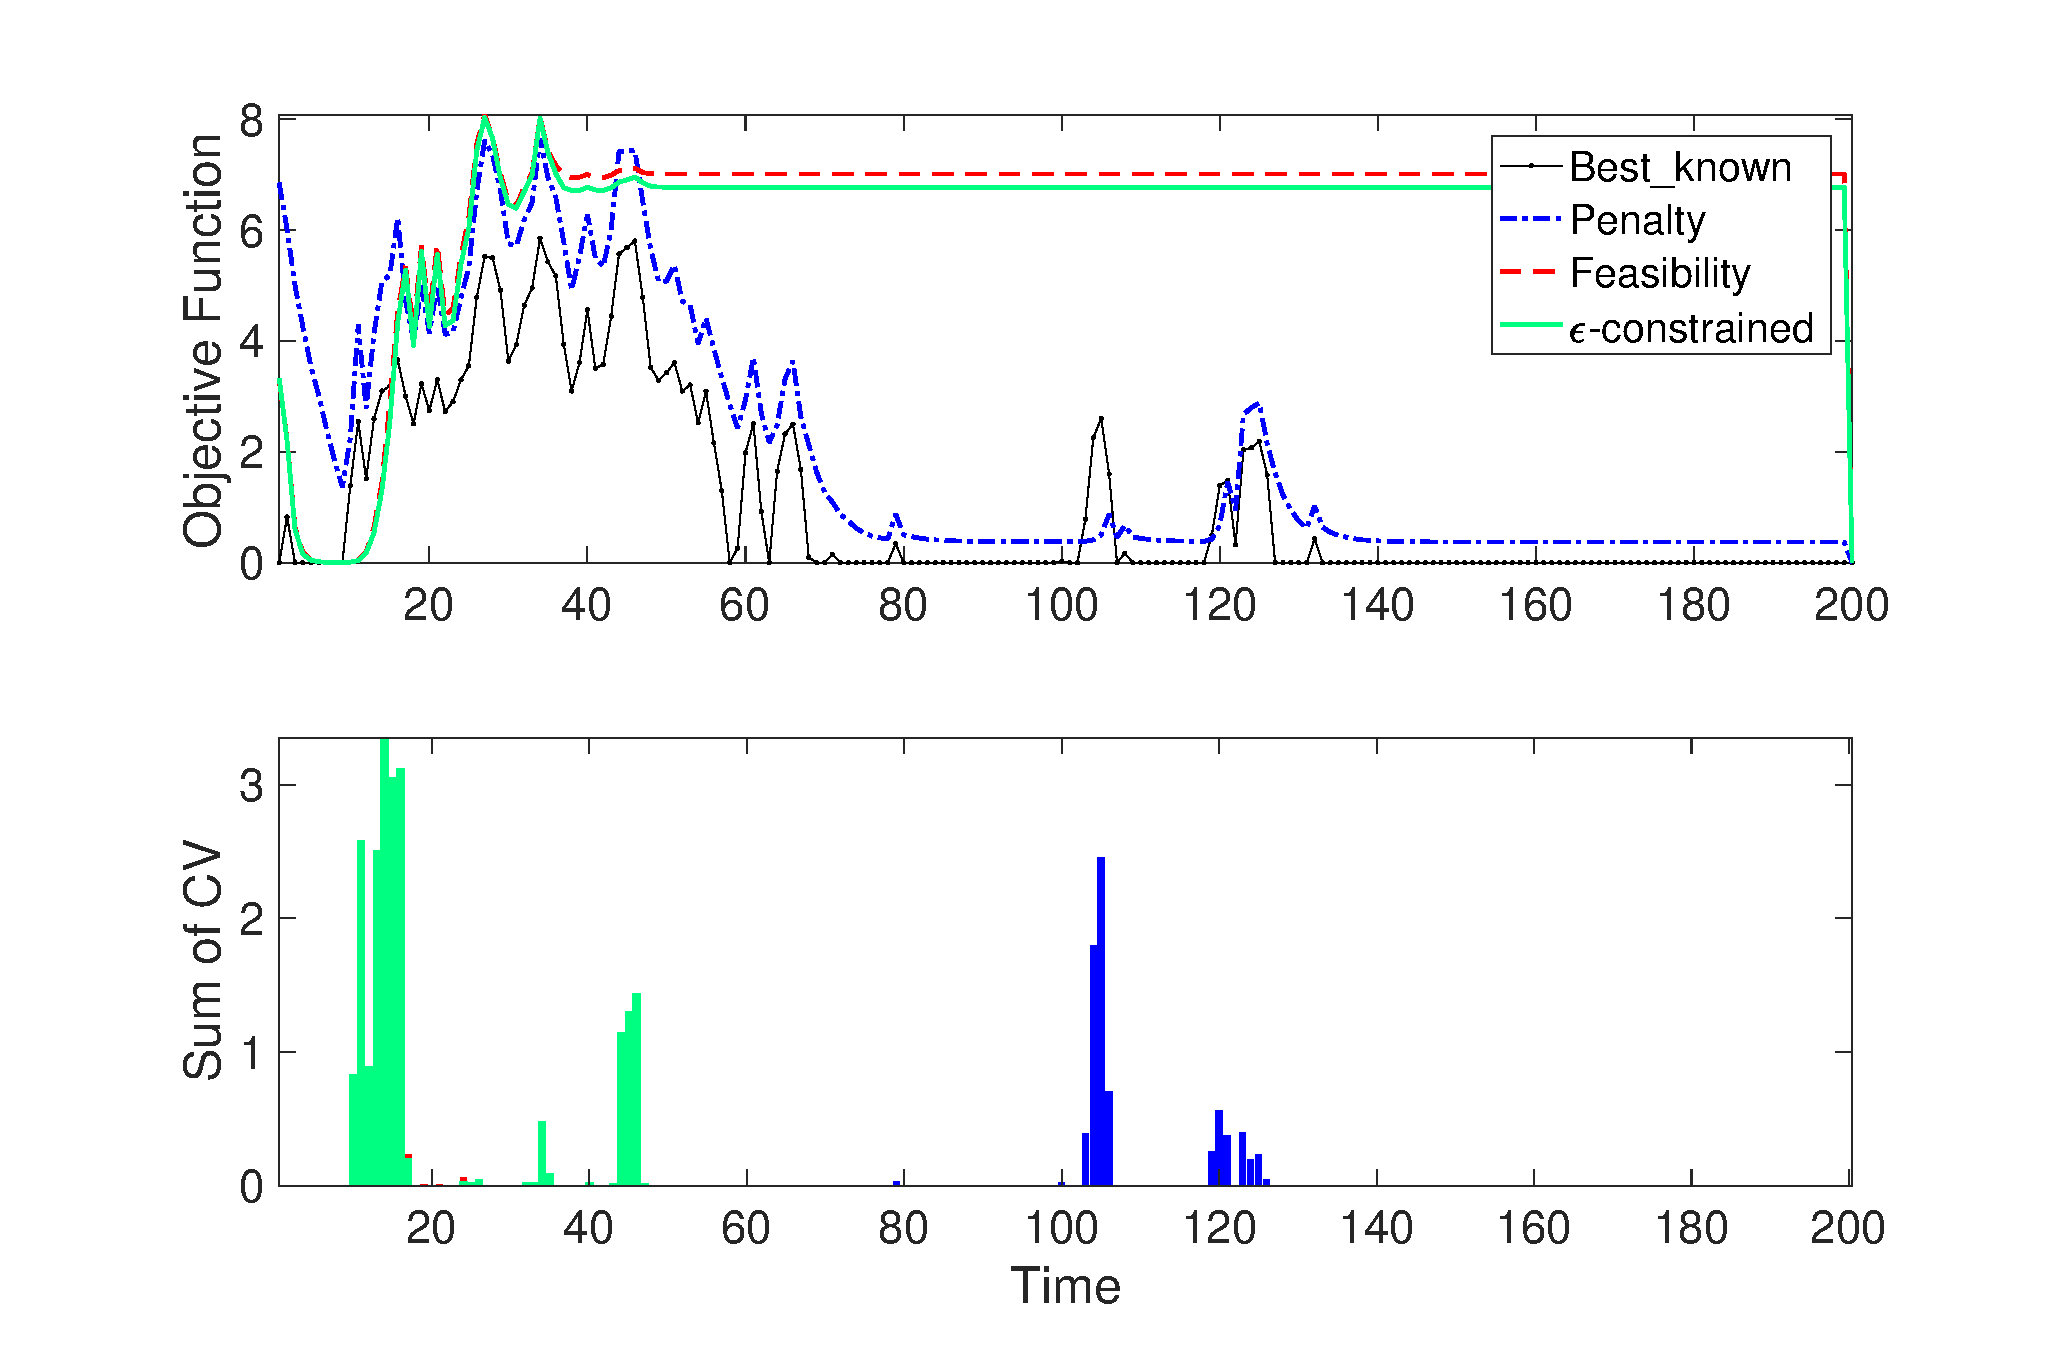
\includegraphics[width=1.1\textwidth, height=6cm]{figs/Ackleyfull.eps}  
        \caption[]
        {\small  Ackley: hyperplane translation (average of 30 runs)} 
        \label{fig:objwCV}
    \end{figure*}
  \begin{figure*}[t!]
        \centering          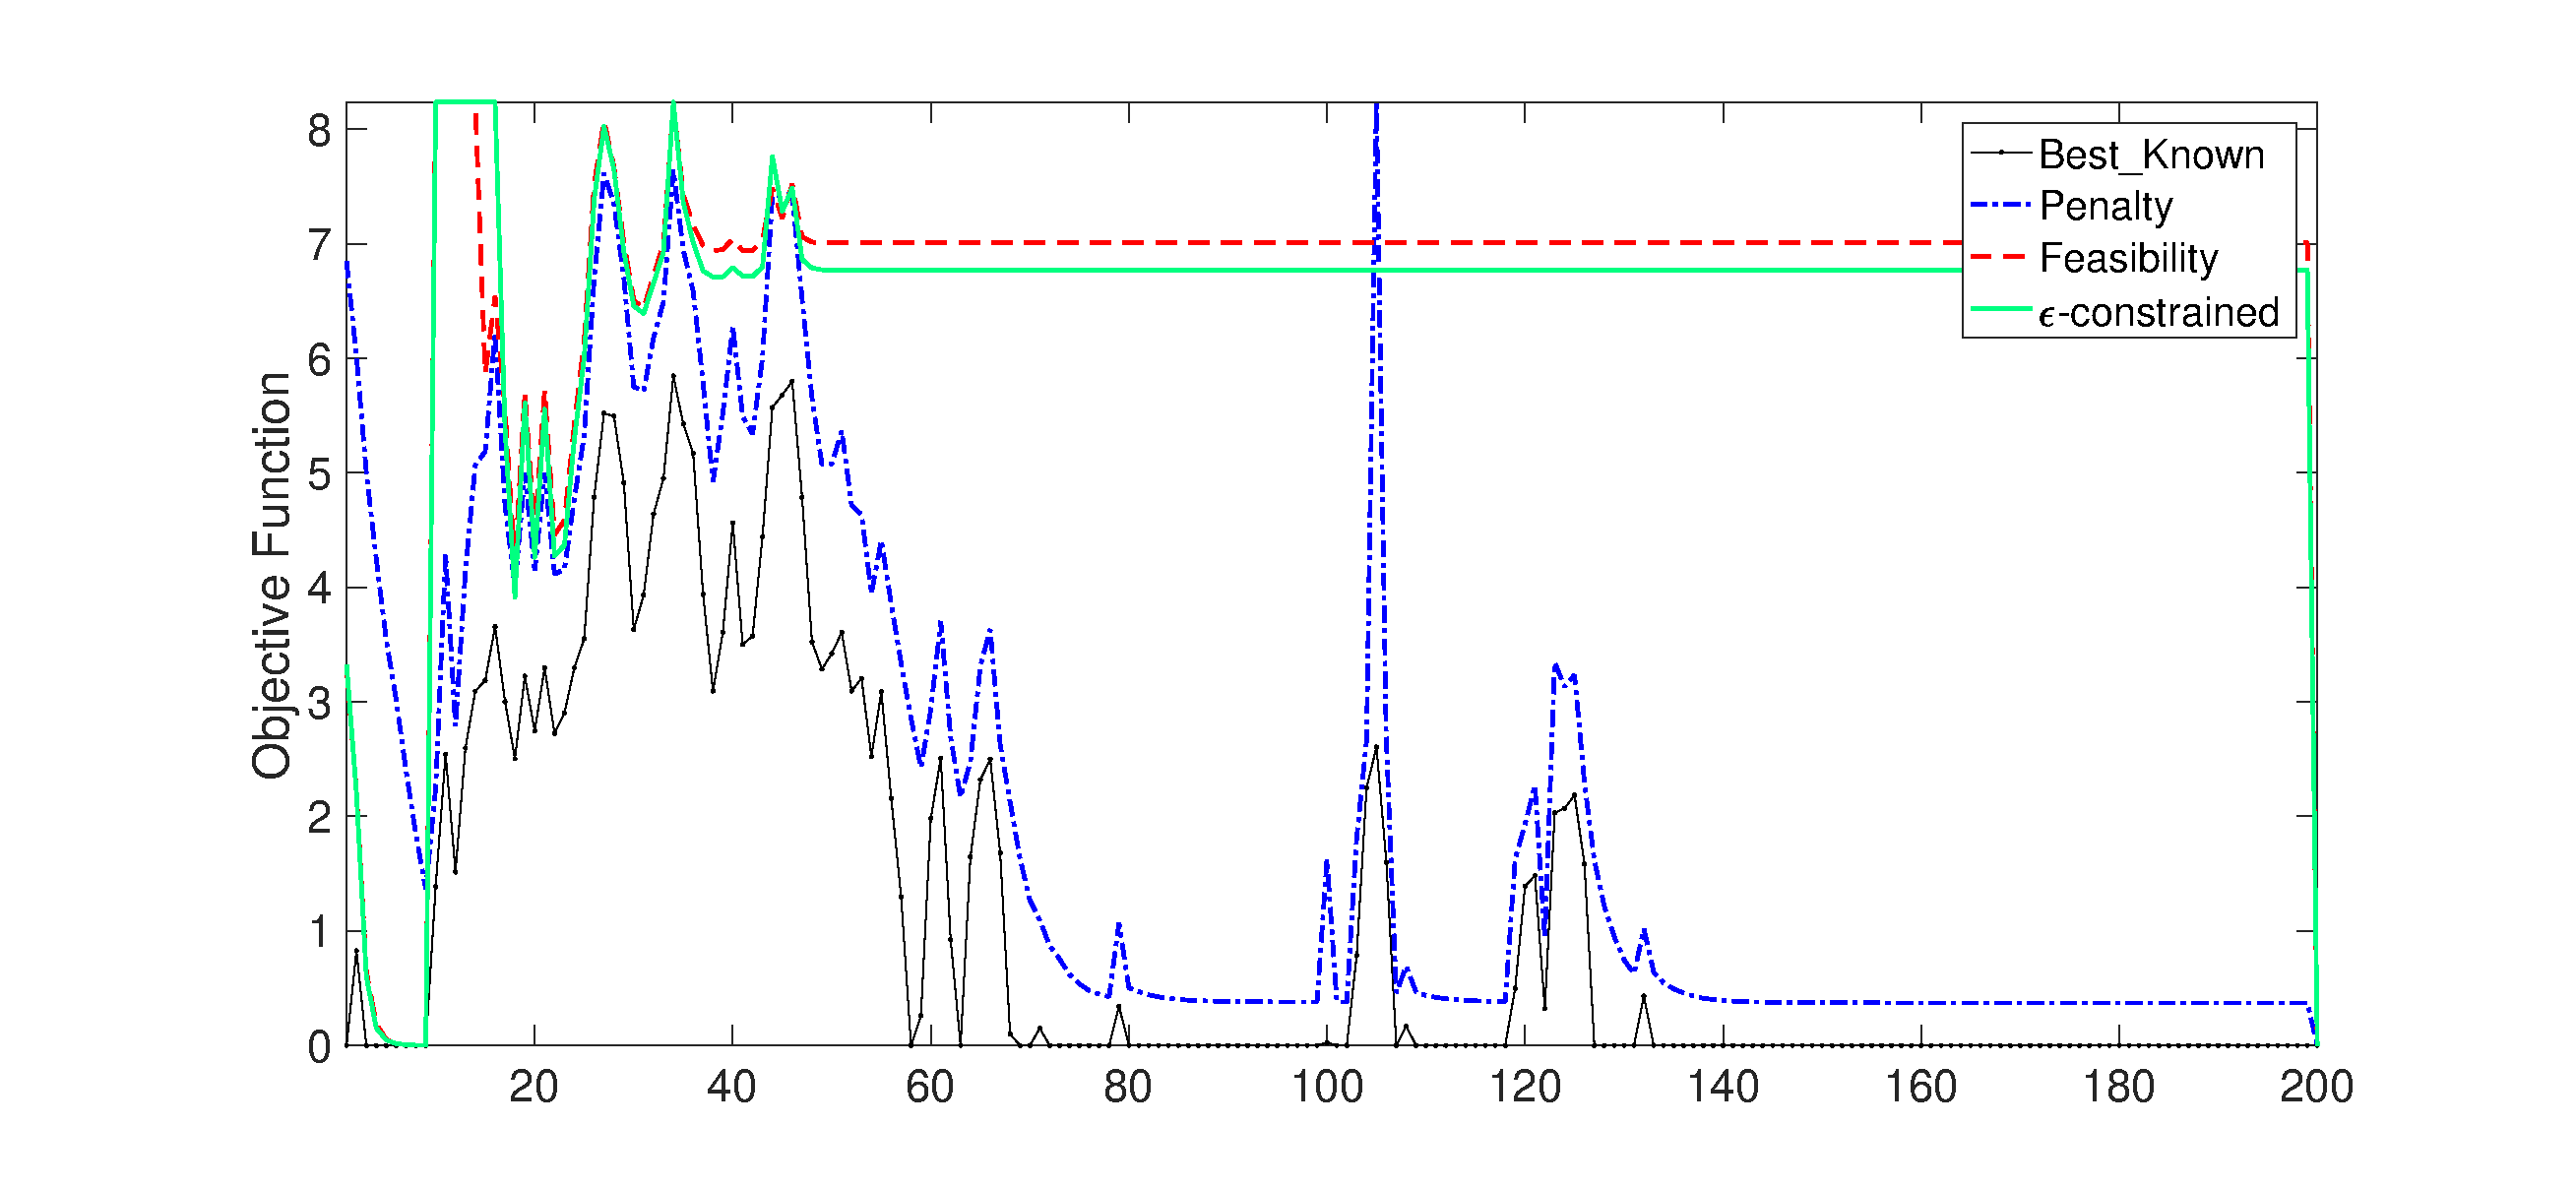
\includegraphics[width=1.1\textwidth, height=6cm]{figs/Ackleypen.eps} 
        \caption[]
        {\small  Ackley: penalized objective function (average of 30 runs)}
         \label{fig:Ackleypenalize}
    \end{figure*}


 \begin{figure*}[t!]
        \centering          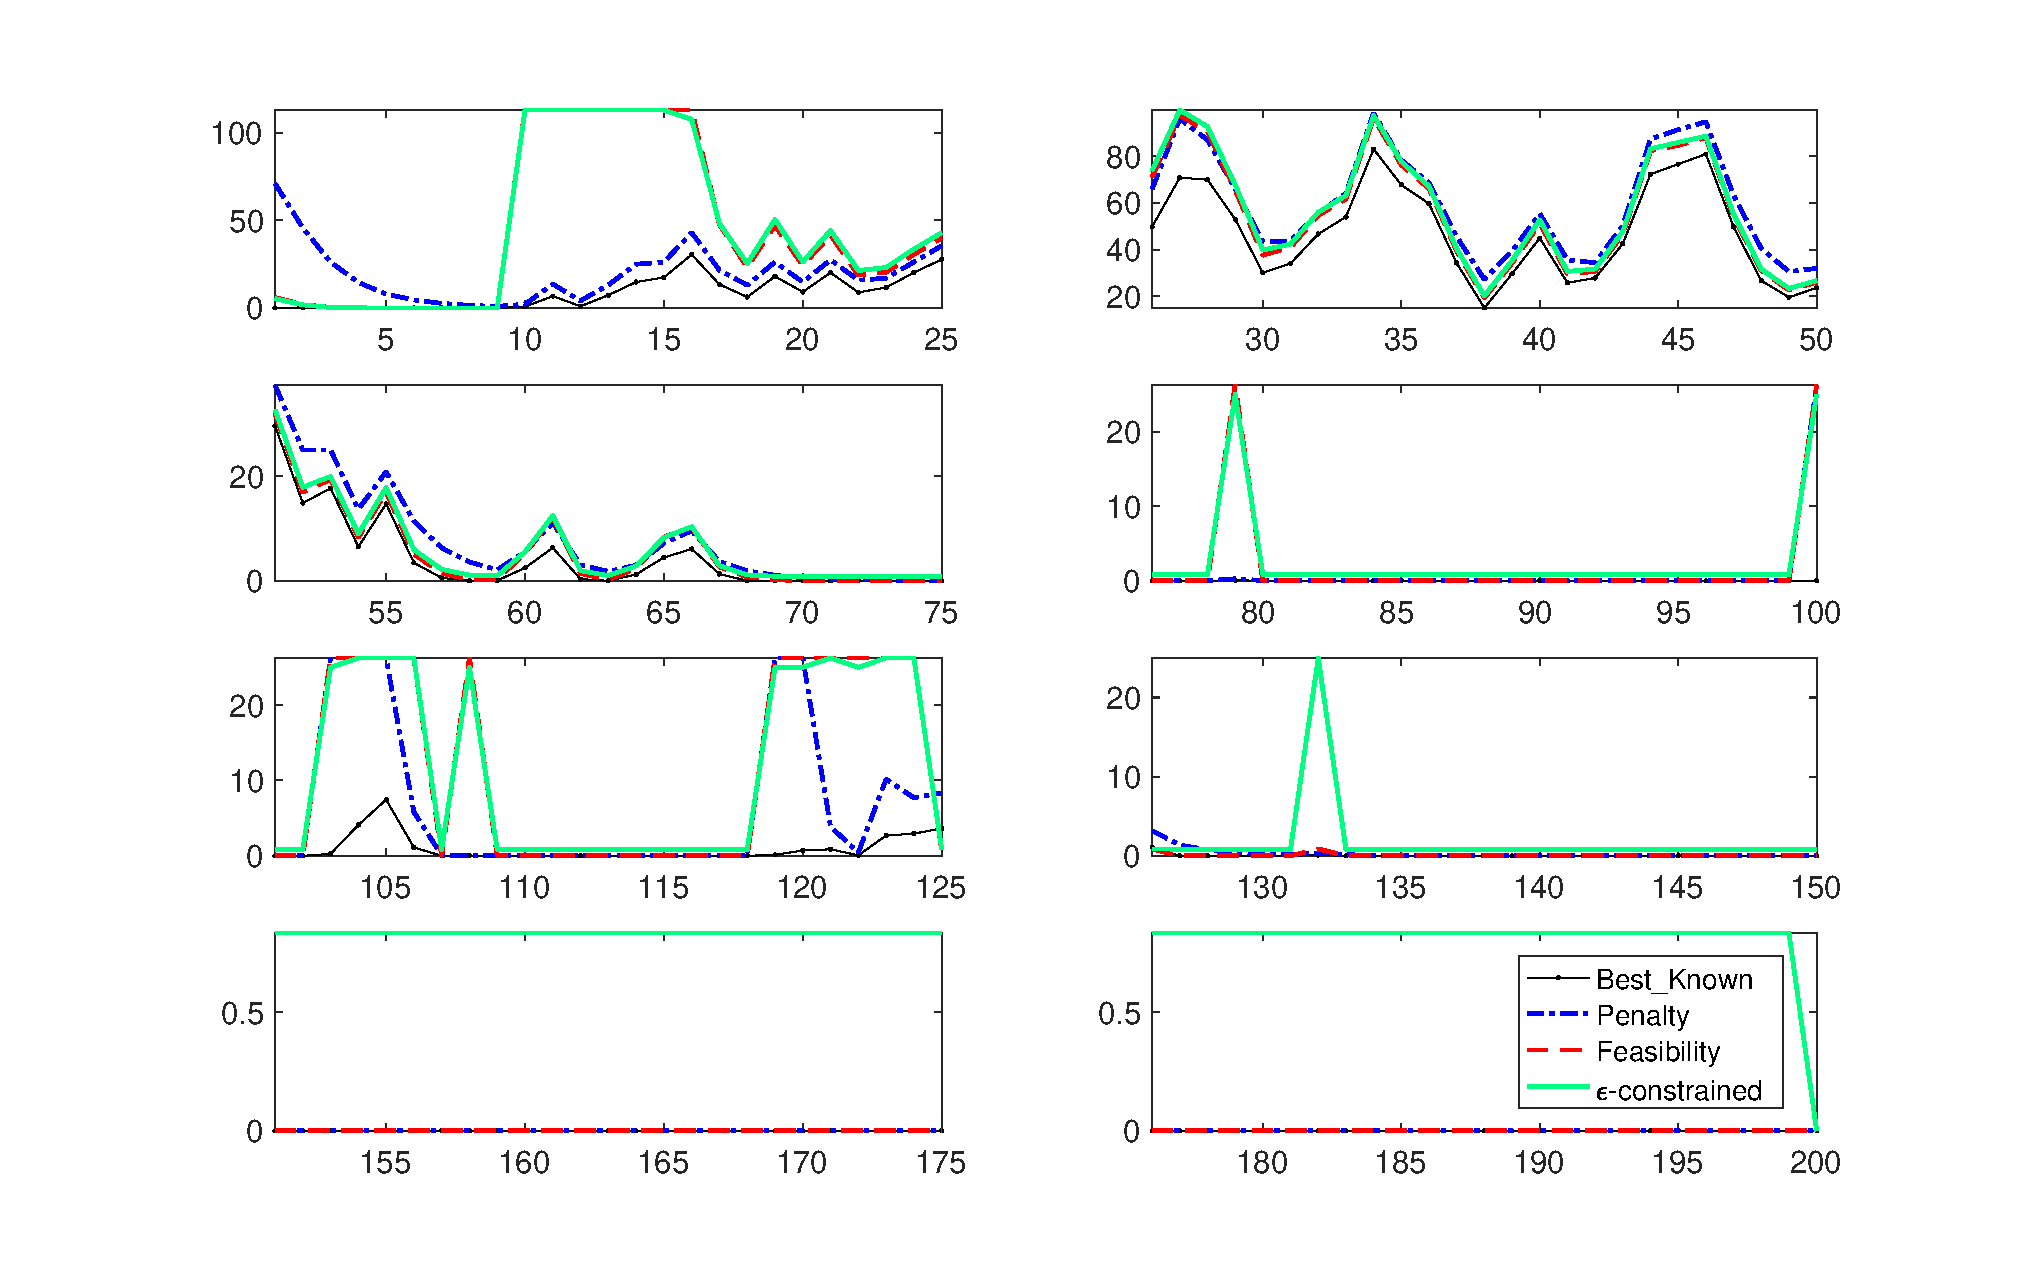
\includegraphics[width=1.1\textwidth, height=6cm]{figs/Sphere8.eps}  
        \caption[]
        {\small  Sphere: hyperplane translation (average of 30 runs)} 
        \label{fig:Sphere8}
    \end{figure*}
    
    
      \begin{figure*}[t!]
        \centering          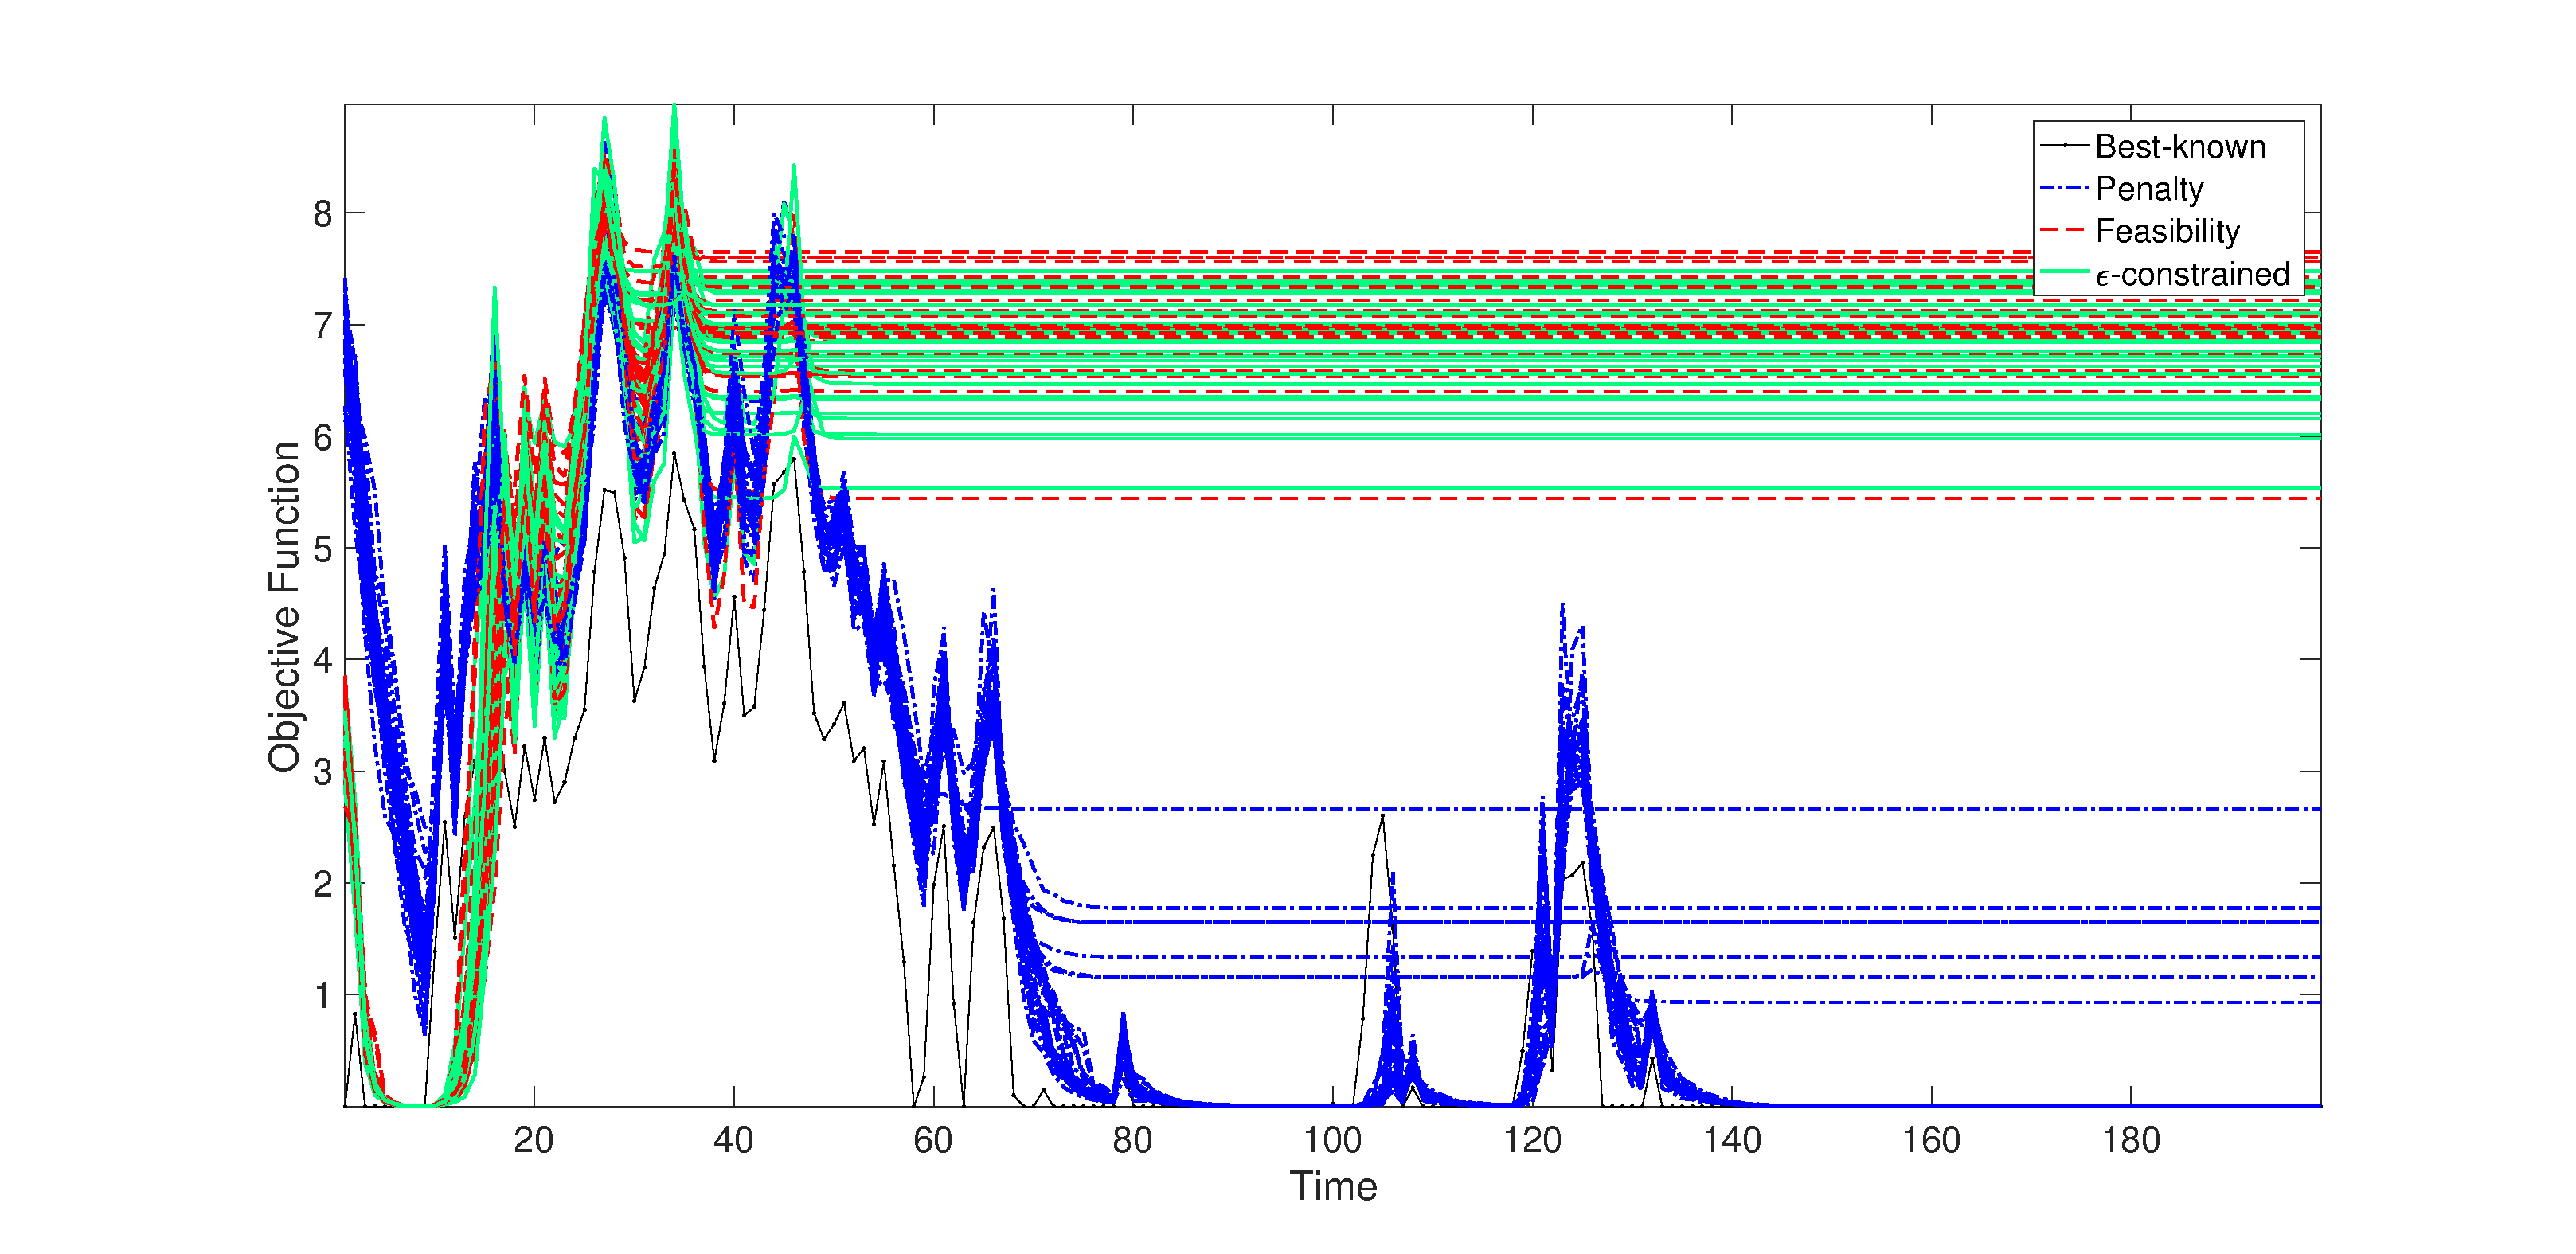
\includegraphics[width=1.1\textwidth, height=6cm]{figs/Ackleyruns.eps} 
        \caption[]
        {\small  Ackley: objective function for all runs}
         \label{fig:Ackleyruns}
    \end{figure*}

\subsubsection{Analysis on analytical test results}
A sample of results (25 times out of 200) for applying the sphere function with a single constraint in the benchmark

The benchmark ran the artificial functions (sphere, Rastrigin, Ackley, \& Rosenbrock) for 200 changes with a single dynamic linear constraint. A sample of the results (25 times) are presented in Table~\ref{tab:singlecons}. As the table shows, the hyperplane translation ($b$\_values) changes the size of the feasible region\footnote{The feasible region is calculated by creating a huge number of individuals randomly and count whether they are feasible} inside of the search space. In this case there is an inverse relation between the size of the feasible region for the sphere function and $b$\_value that is observable in the results. As the feasible region changes over time, new optimal points can appear, represented in the table as best\_known. The way the algorithms track these new best-known solutions is recorded across all of the runs and then the distribution is measured in the table. This allows a comparison between algorithms for specific times, although, for larger time scales individual comparisons are not preferable. The sum of constraint violations was omitted from this table because for almost all of the cases, the algorithms reached feasible solutions for all runs with exception on time 60 (is highlighted with an asterisk in the table), to have infeasible solutions for almost over 50\% of the overall runs.
Table~\ref{tab:powersys} shows similar information to the previous table where a real-world problem (power system) is applied. In a real world problem, a powerful algorithm is required to find robust results. The algorithms implemented to test this benchmark are simple and this lead to the high variance in the optimized solutions present in the table. However, the algorithms still manage to adapt to the dynamism and produce results that approach optimal values. Constraint violations were present in most of the solutions and this was measured in the table. This can be attributed to the existence of equality constraints in the constraint set (see Table~\ref{tab:Constraints}).
\subsubsection{Statistical test results}
For measuring performance of the algorithms across the entire time-scale, we applied two measures, where the results are summarized in Table~\ref{tab:stat}. To validate the results, the 95\%-confidence Kruskal-Wallis statistical test and the Bonferroni post hoc test, as suggested in~\citep{Derrac20113} are presented. Non-parametric tests were adopted because the samples of runs did not fit to a normal distribution based on the Kolmogorov-Smirnov test.
The results of statistical tests showed in almost of the cases with a few exceptions, penalty has significant difference with the other two methods based on modified offline error ($\text{M\_off}\_e$) values. The exceptions are highlighted with an asterisk beside the setting in which we observed a different trend. As in Table~\ref{tab:stat} is illustrated, for Ackley function for experiment 1 (only for medium setting) and 3 we observe there is not significant difference between methods. For this function, for experiment 2 penalty has only significant different with feasibility rules. Another exception belongs to Rosenbrock function in experiment 2 and also the experiment belonged to power system problem (experiment 5), that we could not observe significant different between any of the methods.

One of the limitations of $\text{M\_off}\_e$ measure is that it is biased against generations where solutions are infeasible. This makes our ranking procedure better suited to dynamic environments because it only uses an algorithm's best solution for each time and considers both criteria (objective value \& sum of constraint violation) in selecting a higher performing result.
As Table~\ref{tab:stat} shows, the analysis conducted in the convergence plots also holds true for the analytical test.
The magnitude of the effect that amplitude has on the performance of the algorithms is greater than the effect that frequency has. The magnitude in difference in $\text{M\_off}\_e$ between the respective small \& large settings was greater for amplitude in every single test case. The reason behind this is that drastic changes lead to early solutions being infeasible or non-optimal.
In the results, some algorithms are ranked higher than others despite having greater observed $\text{M\_off}\_e$. This is caused by the ranking solutions selecting the single best solution for each time and then comparing algorithms, whereas $\text{M\_off}\_e$ is measured per generation. Penalty is competitive with $\epsilon$-constrained across the functions despite usually having a higher $\text{M\_off}\_e$ due to the fact that Penalty accepts more infeasible solutions \& $\text{M\_off}\_e$ picks the worst solution if the best is infeasible. When ranking algorithms the best solution overall for each time is selected and this allows Penalty to rank higher.
For sphere function regardless of the experiment, the algorithms ranked identically relative to each other. Feasibility outperformed the others with Penalty coming second and $\epsilon$-constrained coming last. The power system problem also resulted in these rankings. This trend is also observed in the Rosenbrock function with the only exception being the small frequency setting where $\epsilon$-constrained outperformed Penalty. The other two functions, Rastrigin \& Ackley show a similar trend although there is more variance in the rankings. Penalty and $\epsilon$-constrained are still competitive, however, on some occasions $\epsilon$-constrained becomes competitive with feasibility. There is a single case in Rastrigin where Penalty outranks the other algorithms in the combinatorial experiment.
As the amplitude setting increases, the $\text{M\_off}\_e$ also increases. This is present across all functions. The multiple constraint experiment tends to have higher $\text{M\_off}\_e$ compared to the other single constraint experiments, this is due to the increased difficulty that comes with satisfying multiple constraints at the same time over a single one. The combinatorial tends to have one of the highest $\text{M\_off}\_e$, it is usually beaten by large hyperplane translation and multiple constraints. This is because in this experiment the hyperplane is both translating and rotating. The effect of hyperplane rotation on algorithm performance is lesser than that of translation, this leads to larger translation values affecting performance to a greater degree.
\begin{table*}[t!]
\centering
\caption{Testing benchmark for single constraint setup (sphere function)}
\label{tab:singlecons}
\scalebox{0.7}{
\begin{tabular}{l|l|c|l|l|l|l}
Time& $b$\_Values &          Feasible region(\%) & Best-Known & Penalty & Feasibility & $\epsilon$-constrained                        \\\hline

51 & -5.46 & 97\% & 29.65   & 37.46($\pm$2.45)   & 32.04  ($\pm$0.54)    & 32.73($\pm$3.10)   \\
52  & -3.86 & 90\% & 14.87   & 25.02($\pm$4.60)    & 16.99    ($\pm$0.40)    & 17.89($\pm$3.39) \\
53 & -4.22 & 92\% & 17.70     & 25.049($\pm$2.9546)   & 19.382   ($\pm$0.37)    & 19.97($\pm$3.38)  \\
54 & -2.55 & 81\% & 6.50   & 13.70($\pm$2.24)   & 8.30   ($\pm$0.41)    & 8.99($\pm$3.77)  \\
55 & -3.84 & 90\% & 14.72   & 20.86($\pm$2.50)    & 16.98    ($\pm$0.42)    & 17.85($\pm$3.45)  \\
56 & -1.86 & 73\% & 3.45   & 11.40($\pm$ 3.35)   & 5.13   ($\pm$0.36)    & 5.94($\pm$3.98)  \\
57 & -0.75 & 60\% & 0.57  & 6.30($\pm$1.76)   & 1.44   ($\pm$0.19)    & 2.19($\pm$4.37)  \\
58 & 0.50 & 43\% & 0.00        & 3.59($\pm$0.94)  & 0.30   ($\pm$0.16)    & 1.10($\pm$4.53)  \\
59 & -0.23 & 53\% & 0.05 & 2.11($\pm$0.58)  & 0.17   ($\pm$0.07)   & 0.98($\pm$4.54)  \\
60$^*$ & -1.58 & 70\% & 2.48   & 5.57($\pm$1.06)   & 5.16     ($\pm$1.35)     & 5.70($\pm$4.08)  \\
61 & -2.52 & 80\% & 6.31   & 11.11($\pm$1.73)   & 12.11   ($\pm$2.39)     & 12.45($\pm$4.19)  \\
62 & -0.57 &57\% & 0.33   & 3.04($\pm$0.81)  & 1.41   ($\pm$0.88)    & 1.91($\pm$4.45)  \\
63 & 0.59  & 41\% & 0.00        & 1.79($\pm$0.57)  & 0.22   ($\pm$0.19)    & 1.012($\pm$4.54)  \\
64 & -1.115 & 65\% & 1.24   & 2.97($\pm$0.43)  & 2.39  ($\pm$1.51)       & 2.85($\pm$4.21)  \\
65 & -2.12 &76\% & 4.46   & 7.19($\pm$0.76)  & 8.37   ($\pm$3.72)     & 8.28($\pm$3.86)  \\
66 & -2.47 & 80\% & 6.09   & 9.58($\pm$1.35)   & 10.28   ($\pm$3.45)     & 10.34($\pm$3.93)  \\
67 & -1.15 & 65\% & 1.31   & 3.68($\pm$0.66)  & 2.68   ($\pm$2.57)     & 2.88($\pm$4.26)    \\
68 & -0.11 & 51\% & 0.01  & 1.92($\pm$0.55)  & 0.75   ($\pm$2.21)     & 1.12($\pm$4.52)  \\
69  & 1.58  & 29\% & 0.00        & 1.04($\pm$0.32)  & 0.21   ($\pm$0.84)    & 0.88($\pm$4.56) \\
70 & 0.89  & 37\% & 0.00        & 0.61($\pm$0.25)  & 0.01 ($\pm$0.02)    & 0.84($\pm$4.56)   \\
71 & -0.15 & 52\% & 0.02 & 0.45($\pm$0.15)  & 0.04 ($\pm$0.01)   & 0.87($\pm$4.55)   \\
72 & 1.29  & 32\%  & 0.00        & 0.24($\pm$0.10) & 0.01($\pm$0.01)  & 0.84($\pm$4.56) \\
73 & 2.83  & 16\%  & 0.00        & 0.12($\pm$0.04) & 0.00 ($\pm$0.00)  & 0.83($\pm$4.56) \\
74 & 1.06  & 35\% & 0.00        & 0.07($\pm$0.03) & 0.00($\pm$0.00)  & 0.83($\pm$4.56)  \\
75 & 3.03  & 14\% & 0.00        & 0.04($\pm$0.02) & 0.00($\pm$0.00) & 0.83($\pm$4.56) 
\end{tabular}
}
\end{table*}

 

\begin{table*}[t!]
\centering
\caption{Testing benchmark on power system problem}
\label{tab:powersys}
\scalebox{0.7}{
\begin{tabular}{l|c|l|l|l|l|l|l}
Time & Best\_known & Penalty      & Feasibility  & $\epsilon$-constrained  & Penalty\_cv  & Feasibility\_cv & $\epsilon$-constrained\_cv \\
1    & 6410               &  10690($\pm$4077)& 11156($\pm$2417)    & 11061($\pm$2693)  & 48.16 ($\pm$23.68)   & 0.99($\pm$0.65)     & 1.09($\pm$ 0.70)    \\
2    & 6756          & 8191($\pm$2390)   & 10622($\pm$2609)    & 10872($\pm$2034)  & 7.50($\pm$8.06)   & 0.42($\pm$0.41)    & 0.49($\pm$0.43)    \\
3    & 6854                & 8866($\pm$2752) & 11033($\pm$3079)    & 10345($\pm$2328)  & 1.86($\pm$3.28)   & 0.23($\pm$0.30)     & 0.27($\pm$0.36)    \\
4    & 8017                   & 9205($\pm$3233) & 10230($\pm$3104)    & 9605($\pm$2527)  & 1.60($\pm$3.34)    & 0.12($\pm$0.22)     & 0.11($\pm$0.18)    \\
5    & 6039                   & 9614($\pm$3706) & 11003($\pm$3205)    & 9015($\pm$2367)  & 1.30($\pm$3.14)   & 0.09($\pm$0.17)     & 0.09($\pm$0.16)    \\
6    & 5083                   & 8927($\pm$3443) & 10589($\pm$3210)    & 9808($\pm$3002)    & 1.31($\pm$3.24)   & 0.16($\pm$ 0.20)     & 0.19($\pm$0.32)    \\
7    & 5189                 & 9121($\pm$3069) & 10416($\pm$2682)    & 10278($\pm$2594)  & 0.53($\pm$0.42)  & 0.23($\pm$0.25)     & 0.20($\pm$0.22)    \\
8    & 6255                    & 9696($\pm$3845) & 9413($\pm$2547)    & 9439($\pm$2311)  & 0.30($\pm$0.42)  & 0.05($\pm$0.12)     & 0.05($\pm$0.11)    \\
9    & 6535                     & 9436($\pm$3235) & 9059($\pm$2517)    & 9052($\pm$3349)  & 0.23($\pm$0.41)  & 0.01($\pm$0.04)    & 0.02($\pm$0.07)   \\
10   & 6179                 & 9265($\pm$3360) & 9702($\pm$2902)    & 9669($\pm$2389)  & 0.70($\pm$0.95)   & 0.05($\pm$0.12)     & 0.06($\pm$0.12)    \\
11   & 6681                      & 8991($\pm$3321) & 9081($\pm$3046)    & 8174($\pm$2075)  & 0.85($\pm$1.27)   & 0.00($\pm$0.00)    & 0.02($\pm$0.08)   \\
12   & 5022                    & 9181($\pm$3054) & 10727($\pm$3326)    & 8973($\pm$2120)  & 3.53($\pm$5.93)   & 0.13($\pm$0.20)     & 0.06($\pm$0.13)    \\
13   & 6149                   & 10064($\pm$3216) & 10480($\pm$2946)    & 9327($\pm$2511)  & 4.26($\pm$7.35)   & 0.10($\pm$0.17)     & 0.06($\pm$0.12)     \\
14   & 7443                  & 9451($\pm$2549) & 10626($\pm$3441)    & 8450($\pm$2410)  & 3.31($\pm$6.13)   & 0.07($\pm$0.15)     & 0.01($\pm$0.06)   \\
15   & 5962              & 9146($\pm$2752) & 9406($\pm$2724)    & 8294($\pm$2437)  & 3.65($\pm$7.05)   & 0.01($\pm$0.05)    & 0.00($\pm$0.00)   \\
16   & 5997                  & 9082($\pm$3043) & 8392($\pm$1676)    & 7302($\pm$1915)  & 3.62($\pm$7.06)   & 0.00($\pm$0.00)           & 0.00($\pm$0.00)          \\
17   & 6947                    & 8984($\pm$2719) & 9980($\pm$2690)    & 8408($\pm$2146)    & 4.21($\pm$4.86)    & 0.02($\pm$0.07)    & 0.01($\pm$0.06)   \\
18   & 6684                  & 9053($\pm$2807) & 8482($\pm$1594)      & 7578($\pm$1963)  & 4.17($\pm$4.89)   & 0.00($\pm$0.00)    & 0.00($\pm$0.00)          \\
19   & 5214                    & 9063($\pm$2886) & 8613($\pm$1748)    & 7989($\pm$2464)  & 6.48($\pm$6.77)   & 0.01($\pm$0.05)    & 0.01($\pm$0.04)   \\
20   & 7027                    & 9029($\pm$2876) & 9367($\pm$2514)    & 7771($\pm$2205)  & 7.13($\pm$7.32)   & 0.02($\pm$0.08)    & 0.01($\pm$0.04)  
\end{tabular}
}
\end{table*}
%%%%%%%table for stat test
 \begin{figure*}[t!]
        \centering          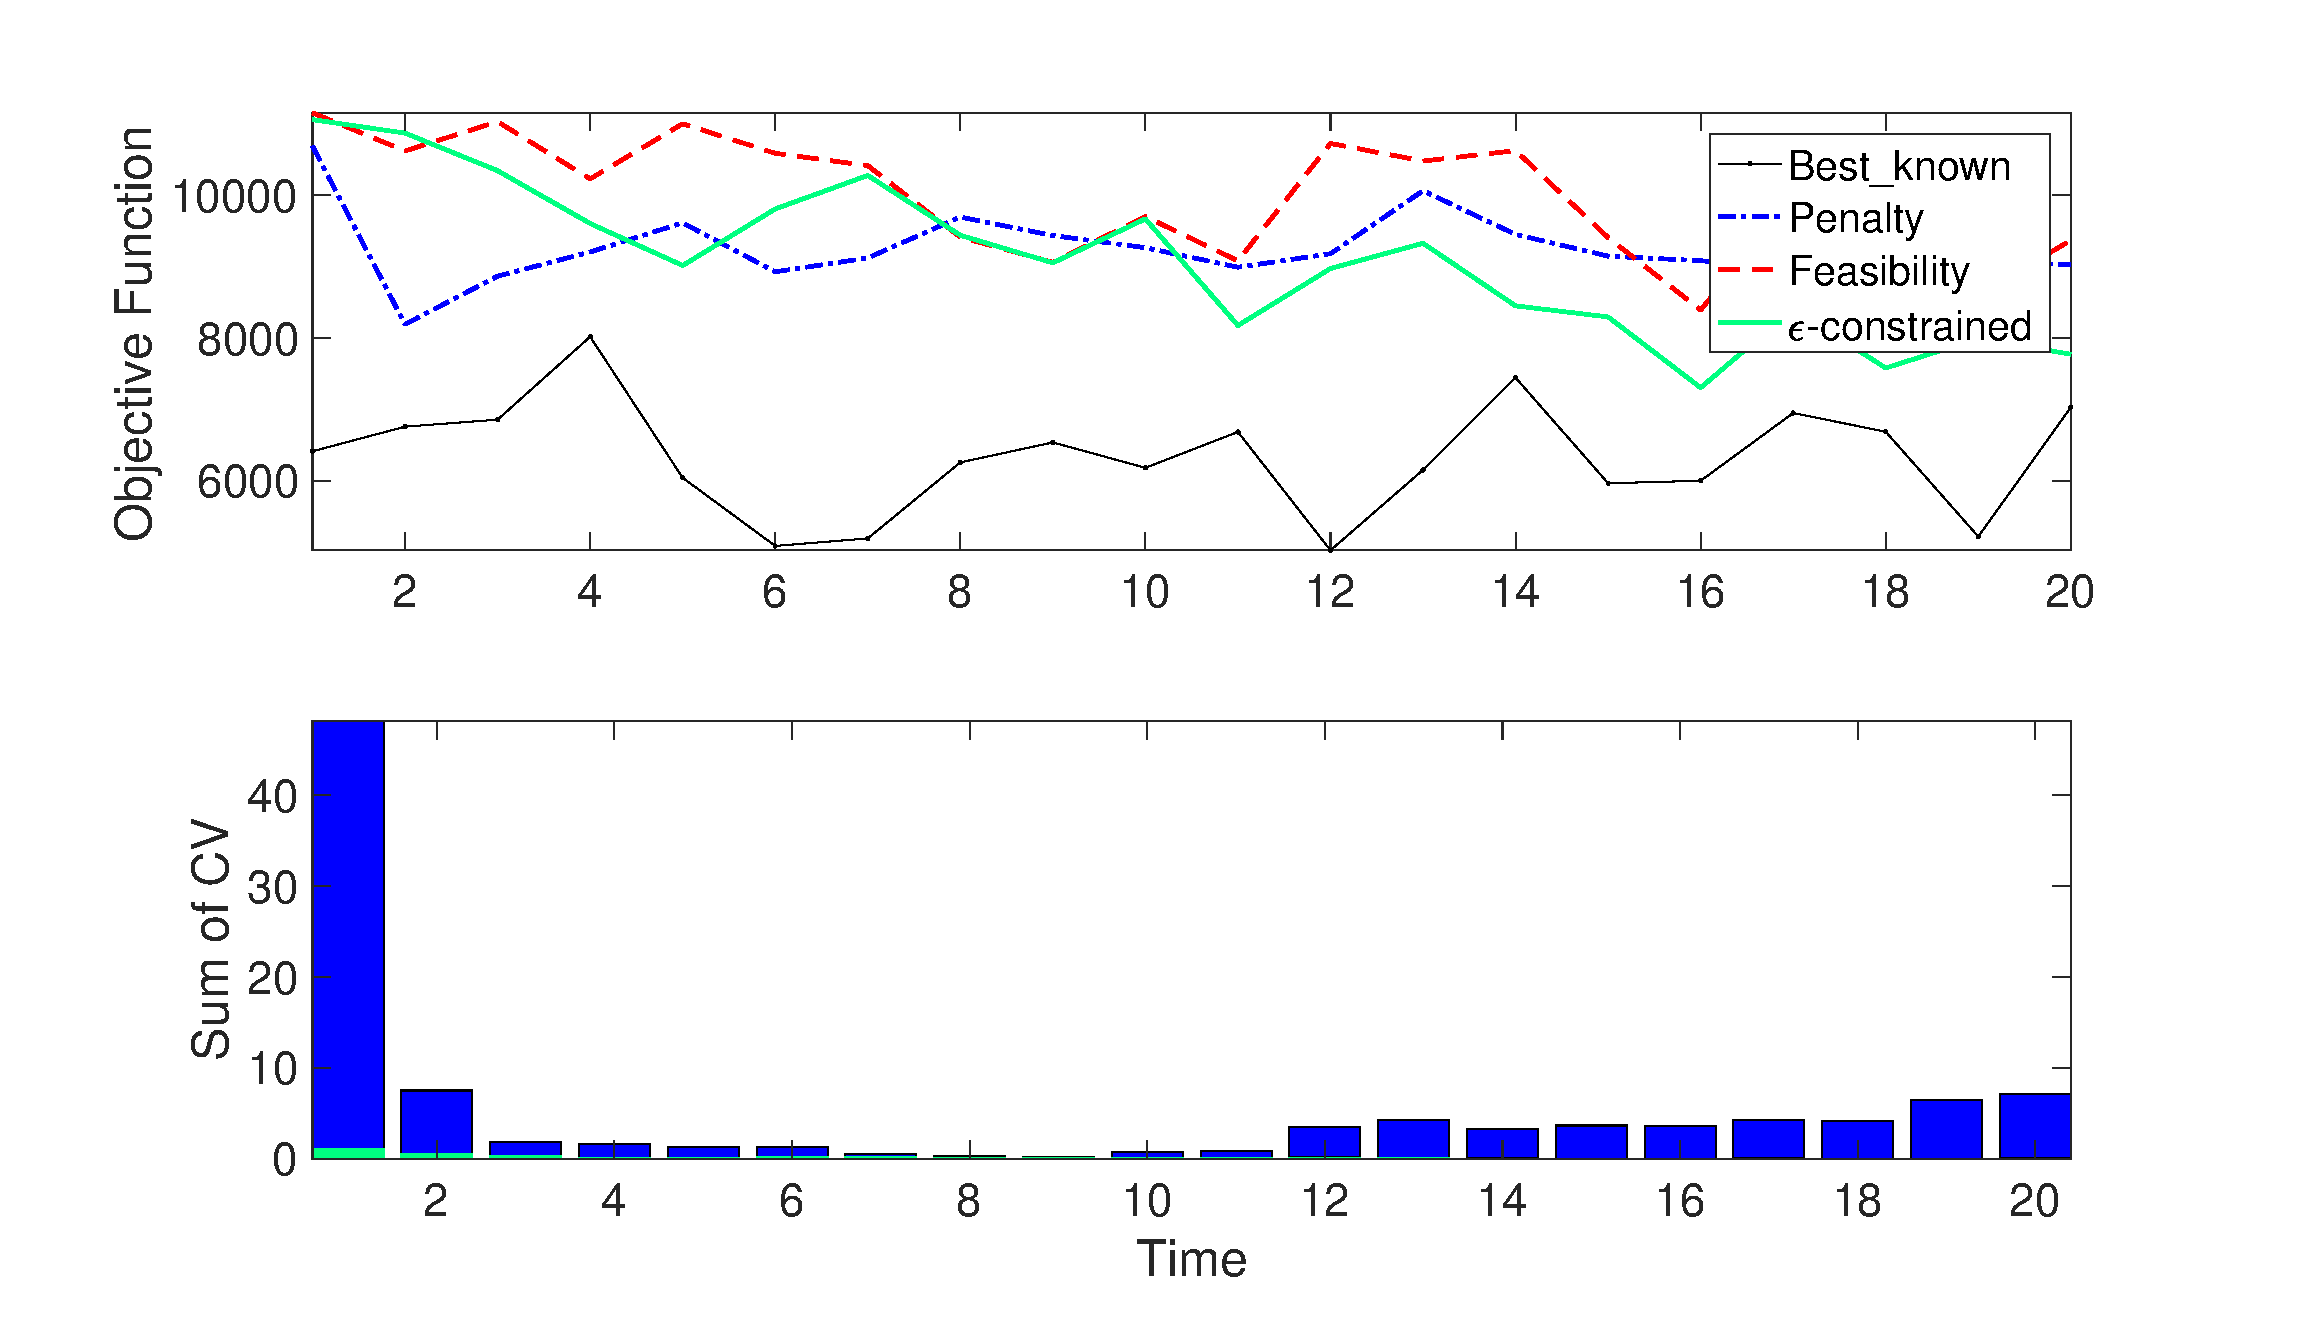
\includegraphics[width=1\textwidth, height=6cm]{figs/powersysresult.eps} 
        \caption[]
        {\small Power system problem-hyperplane translation}
         \label{fig:posysresult}
    \end{figure*}



\begin{table*}[t]
\centering
\caption{Analytical test results}
\label{tab:stat}
\scalebox{0.7}{
\begin{tabular}{cc|llllll}
\hline
\multicolumn{8}{c}{\textbf{Function 1:Sphere}}                                                                                                                                       \\\hline
                                  &        & \multicolumn{2}{l}{Penalty}   & \multicolumn{2}{l}{Feasibility} & \multicolumn{2}{l}{$\epsilon$-Constrained}      \\
                                  &        & Rank & $\text{M\_off\_e}$ & Rank & $\text{M\_off\_e}$   & Rank & $\text{M\_off\_e}$                                \\\hline
                                  & Small  & 2    & 1.97($\pm$0.23)            & 1    & 0.84($\pm$0.05)              & 3    & 0.82($\pm$0.05)                                           \\
Experiment 1: Dynamic b                         & Medium & 2    & 2.52($\pm$0.16)            & 1    & 1.44($\pm$0.27)              & 3    & 1.38($\pm$0.23)                                           \\
                                  & Large  & 2    & 4.97($\pm$0.31)            & 1    & 3.47($\pm$0.47)              & 3    & 4.27($\pm$3.59)                                           \\
\multicolumn{2}{l|}{Experiment 2: Combinatorial}          & 2    & 5.77($\pm$0.90)            & 1    & 3.57($\pm$4.61)              & 3    & 1.92($\pm$0.37)                                           \\
\multicolumn{2}{l|}{Experiment 3: MultipleConst}          & 2    & 30.95($\pm$2.28)           & 1    & 17.98($\pm$5.07)             & 3    & 18.65($\pm$5.80)                                          \\
                                  & Small  & 2    & 3.43($\pm$0.20)            & 1    & 4.89($\pm$6.21)              & 3    & 5.58($\pm$6.91)                                           \\
Experiment 4: Dynamic $\tau$  & Medium & 2    & 4.97($\pm$0.31)            & 1    & 3.47($\pm$0.47)              & 3    & 4.27($\pm$3.59)                                           \\
                                  & Large  & 2    & 7.12($\pm$0.42)            & 1    & 6.13($\pm$5.02)              & 3    & 6.12($\pm$5.07)                                           \\\hline
\multicolumn{8}{c}{\textbf{Function 2:Rastrigin}}                                                                                                                                   \\\hline
                                  &        & \multicolumn{2}{l}{Penalty}   & \multicolumn{2}{l}{Feasibility} & \multicolumn{2}{l}{$\epsilon$-constrained}  \\
                                  &        & Rank & $\text{M\_off\_e}$ & Rank & $\text{M\_off\_e}$   & Rank & $\text{M\_off\_e}$                                \\\hline
                                  & Small  & 2    & 16.54($\pm$2.39)           & 1    & 9.06($\pm$1.15)              & 3    & 8.54($\pm$0.87)                                           \\
Experiment 1: Dynamic b                         & Medium & 2    & 17.99($\pm$2.56)           & 1    & 9.66($\pm$2.07)              & 3    & 9.04($\pm$1.49)                                           \\
                                  & Large  & 3    & 69.51($\pm$15.16)          & 1    & 105.74($\pm$13.91)           & 2    & 102.18($\pm$11.99)                                        \\
\multicolumn{2}{l|}{Experiment 2: Combinatorial}          & 1    & 34.48($\pm$10.13)          & 2    & 11.85($\pm$4.25)             & 3    & 11.27($\pm$2.25)                                          \\
\multicolumn{2}{l|}{Experiment 3: MultipleConst}          & 2    & 91.92($\pm$9.38)           & 1    & 65.48($\pm$10.09)            & 3    & 16.07($\pm$12.96)                                         \\
                                  & Small  & 3    & 92.29($\pm$21.58)          & 1    & 114.30($\pm$17.76)           & 2    & 115.27($\pm$19.23)                                        \\
Experiment 4: Dynamic $\tau$       & Medium & 3    & 69.51($\pm$15.16)          & 1    & 105.74($\pm$13.91)           & 2    & 102.18($\pm$11.99)                                        \\
                                  & Large  & 3    & 68.74($\pm$5.59)           & 2    & 60.97($\pm$11.31)            & 1    & 63.19($\pm$12.63)                                         \\\hline
\multicolumn{8}{c}{\textbf{Function 3:Ackley}}                                                                                                                                      \\\hline
                                  &        & \multicolumn{2}{l}{Penalty}   & \multicolumn{2}{l}{Feasibility} & \multicolumn{2}{l}{$\epsilon$-constrained}  \\
                                  &        & Rank & $\text{M\_off\_e}$ & Rank & $\text{M\_off\_e}$   & Rank & $\text{M\_off\_e}$                                \\
                                  & Small  & 2    & 0.52($\pm$0.02)            & 1    & 0.40($\pm$0.00)              & 3    & 0.40($\pm$0.00)                                           \\
Experiment 1: Dynamic b                         & Medium$^*$ & 3    & 0.90($\pm$0.09)            & 1    & 0.93($\pm$0.09)              & 2    & 0.96($\pm$0.22)                                           \\
                                  & Large  & 3    & 1.09($\pm$0.38)            & 2    & 5.52($\pm$0.38)              & 1    & 5.32($\pm$0.40)                                           \\
\multicolumn{2}{l|}{Experiment 2: Combinatorial$^*$}          & 3    & 2.02($\pm$0.15)            & 1    & 1.98($\pm$0.46)              & 2    & 1.98($\pm$0.33)                                           \\
\multicolumn{2}{l|}{Experiment 3: MultipleConst$^*$}          & 3    & 4.43($\pm$0.09)            & 1    & 4.38($\pm$0.51)              & 2    & 4.37($\pm$0.48)                                           \\
                                  & Small  & 3    & 1.66($\pm$0.79)            & 2    & 5.50($\pm$0.26)              & 1    & 5.45($\pm$0.39)                                           \\
Experiment 4: Dynamic $\tau$       & Medium & 3    & 1.09($\pm$0.38)            & 2    & 5.52($\pm$0.38)              & 1    & 5.32($\pm$0.40)                                           \\
                                  & Large  & 3    & 1.20($\pm$0.90)            & 1    & 3.52($\pm$0.90)              & 2    & 3.40($\pm$0.90)                                           \\\hline
\multicolumn{8}{c}{\textbf{Function 4: Rosenbrock}}                                                                                                                                 \\
                                  &        & \multicolumn{2}{l}{Penalty}   & \multicolumn{2}{l}{Feasibility} & \multicolumn{2}{l}{$\epsilon$-constrained}  \\
                                  &        & Rank & $\text{M\_off\_e}$ & Rank & $\text{M\_off\_e}$   & Rank & $\text{M\_off\_e}$                                \\\hline
                                  & Small  & 2    & 1502.30($\pm$195.00)       & 1    & 880.60(461.50)           & 3    & 846.70($\pm$563.90)                                       \\
Experiment 1: Dynamic b                         & Medium & 2    & 1549.50($\pm$239.10)       & 1    & 3930.10($\pm$9653.90)        & 3    & 3489.80($\pm$9341.50)                                     \\
                                  & Large  & 2    & 3736.60($\pm$499.50)       & 1    & 4852.20($\pm$536.36)         & 3    & 4698.60($\pm$9378.60)                                     \\
\multicolumn{2}{l|}{Experiment 2: Combinatorial$^*$}          & 2    & 3093.00($\pm$385.00)       & 1    & 6818.00($\pm$10440.00)       & 3    & 4762.00($\pm$7598.00)                                     \\
\multicolumn{2}{l|}{Experiment 3: MultipleConst}          & 2    & 2278.90($\pm$3792.00)      & 1    & 1378.00($\pm$8893.00)        & 3    & 12274.00($\pm$8060.00)                                    \\
                                  & Small  & 3    & 2487.30($\pm$456.50)       & 1    & 1929.30($\pm$1070.20)        & 2    & 1708.50($\pm$627.30)                                      \\
Experiment 4: Dynamic $\tau$       & Medium & 2    & 3736.60($\pm$499.50)       & 1    & 4852.20($\pm$536.36)         & 3    & 4698.60($\pm$9378.60)                                     \\
                                  & Large  & 2    & 5906.90($\pm$576.30)       & 1    & 3760.10($\pm$493.50)         & 3    & 3717.70($\pm$413.50)                                      \\\hline
\multicolumn{8}{c}{\textbf{Power system problem}}                                                                                                                                   \\\hline
 Experiment 5$^*$              &         & \multicolumn{2}{l}{Penalty}   & \multicolumn{2}{l}{Feasibility} & \multicolumn{2}{l}{$\epsilon$-constrained}  \\
                                  &        & Rank & $\text{M\_off\_e}$ & Rank & $\text{M\_off\_e}$   & Rank & $\text{M\_off\_e}$                                \\\hline
                                  &        & 2    & 5891.70($\pm$3306.80)      & 1    & 5143.60($\pm$1771.50)         & 3    & 4200.30($\pm$1639.70)                                      \\
\end{tabular}
}
\end{table*}

\section{Conclusion and future work} \label{sec:conclusion}
In this paper a framework has been proposed to generate benchmarks for testing algorithms in DCOPs. Our proposed framework can produce multiple benchmarks to be applied for testing any function and for any number of changes and dimension in the optimization problem. The changes in the environment are imposed by translation and rotation of the hyperplane in single and multiple linear constraints.
For testing our benchmark, three constraint handling techniques have been applied and compared (penalty, feasibility and $\epsilon$-constrained) with differential evolutionary algorithm. A procedure for ranking the algorithms that is based on the feasibility rules was proposed to analyze the results and compare the algorithms behaviour.
Implementing a range of artificial functions and one real-world example in power systems domain proofed that our proposed benchmark can be applied to any function effectively.
While the behavior of the used techniques was similar, the performance had a higher dependency on the amplitude than the frequency however, they both had an effect on the fitness and constraint violations. 
For future work the proposed benchmark would need to be tested with more advanced algorithms. The current constraint handling techniques struggle with dynamism so these algorithms will need to be designed for the dynamic environment. 

\section*{References}

\bibliography{mybibfile}

\end{document}